\documentclass[12pt, oneside]{article}

\usepackage[letterpaper, scale=0.8, centering]{geometry}
\usepackage{fancyhdr}
\setlength{\parindent}{0em}
\setlength{\parskip}{1em}

\pagestyle{fancy}
\fancyhf{}
\renewcommand{\headrulewidth}{0pt}
\rfoot{{\footnotesize Copyright Mia Minnes, 2024, Version \today~(\thepage)}}

\usepackage{titlesec}

\author{CSE20S24}

\newcommand{\instructions}{{\bf For all HW assignments:} 
These homework assignments may be done individually or in groups of up to 3 students.
Please ensure your name(s) and PID(s)
are clearly visible on the first page of your homework
submission, start each question on a new page, and upload the PDF to Gradescope.
If you're working in a group, {\it submit only one submission per group}: one partner uploads the
submission through their Gradescope account and then adds the other group member(s) to the Gradescope submission
by selecting their name(s) in the ``Add Group Members'' dialog box. You will need to re-add your group member(s)
every time you resubmit a new version of your assignment.

Each homework question will be graded either for
{\bf correctness} (including clear and precise explanations and justifications of all answers) or
{\bf fair effort completeness}. You may collaborate on ``graded for correctness''
questions only with CSE 20 students in your group; if your
 group has questions about a problem, you may ask in drop-in help hours or post a private
post (visible only to the Instructors) on Piazza.  
 For ``graded for completeness''
 questions: collaboration is allowed with any CSE 20 students this quarter; 
 if your group has questions about a problem, you may ask in drop-in 
 help hours or post a public post on Piazza.

All submitted homework for this class must be typed. 
You can use a word processing editor if you like (Microsoft Word, Open Office, Notepad, Vim, Google Docs, etc.) 
but you might find it useful to take this opportunity to learn LaTeX. 
LaTeX is a markup language used widely in computer science and mathematics. 
The homework assignments are typed using LaTeX and you can use the source files 
as templates for typesetting your solutions.

{\bf Integrity reminders}
\begin{itemize}
\item Problems should be solved together, not divided up between the partners. The homework is
designed to give you practice with the main concepts and techniques of the course, 
while getting to know and learn from your classmates.
\item You may not collaborate on homework questions graded for correctness with anyone other than your group members.
You may ask questions about the homework in office hours (of the instructor, TAs, and/or tutors) and 
on Piazza (as private notes viewable only to the Instructors).  
You \emph{cannot} use any online resources about the course content other than the class material 
from this quarter -- this is primarily to ensure that we all use consistent notation and
definitions (aligned with the textbook) and also to protect the learning experience you will have when
the `aha' moments of solving the problem authentically happen.
\item Do not share written solutions or partial solutions for homework with 
other students in the class who are not in your group. Doing so would dilute their learning 
experience and detract from their success in the class.
\end{itemize}

}

\newcommand{\gradeCorrect}{({\it Graded for correctness}) }
\newcommand{\gradeCorrectFirst}{\gradeCorrect\footnote{This means your solution 
will be evaluated not only on the correctness of your answers, but on your ability
to present your ideas clearly and logically. You should explain how you 
arrived at your conclusions, using
mathematically sound reasoning. Whether you use formal proof techniques or 
write a more informal argument
for why something is true, your answers should always be well-supported. 
Your goal should be to convince the
reader that your results and methods are sound.} }
\newcommand{\gradeComplete}{({\it Graded for completeness}) }
\newcommand{\gradeCompleteFirst}{\gradeComplete\footnote{This means you will 
get full credit so long as your submission demonstrates honest effort to 
answer the question. You will not be penalized for incorrect answers. 
To demonstrate your honest effort in answering the question, we 
expect you to include your attempt to answer *each* part of the question. 
If you get stuck with your attempt, you can still demonstrate 
your effort by explaining where you got stuck and what 
you did to try to get unstuck.} }

%\usepackage{tikz}
%\usetikzlibrary{circuits.logic.US,circuits.logic.IEC}

\usepackage{amssymb,amsmath,pifont,amsfonts,comment,enumerate,enumitem}
\usepackage{currfile,xstring,hyperref,tabularx,graphicx,wasysym}
\usepackage[labelformat=empty]{caption}
\usepackage{xcolor}
\usepackage{multicol,multirow,array,listings,tabularx,lastpage,textcomp,booktabs}

% NOTE(joe): This environment is credit @pnpo (https://tex.stackexchange.com/a/218450)
\lstnewenvironment{algorithm}[1][] %defines the algorithm listing environment
{   
    \lstset{ %this is the stype
        mathescape=true,
        frame=tB,
        numbers=left, 
        numberstyle=\tiny,
        basicstyle=\rmfamily\scriptsize, 
        keywordstyle=\color{black}\bfseries,
        keywords={,procedure, div, for, to, input, output, return, datatype, function, in, if, else, foreach, while, begin, end, }
        numbers=left,
        xleftmargin=.04\textwidth,
        #1
    }
}
{}
\lstnewenvironment{java}[1][]
{   
    \lstset{
        language=java,
        mathescape=true,
        frame=tB,
        numbers=left, 
        numberstyle=\tiny,
        basicstyle=\ttfamily\scriptsize, 
        keywordstyle=\color{black}\bfseries,
        keywords={, int, double, for, return, if, else, while, }
        numbers=left,
        xleftmargin=.04\textwidth,
        #1
    }
}
{}

\newcommand\abs[1]{\lvert~#1~\rvert}
\newcommand{\st}{\mid}

\newcommand{\A}[0]{\texttt{A}}
\newcommand{\C}[0]{\texttt{C}}
\newcommand{\G}[0]{\texttt{G}}
\newcommand{\U}[0]{\texttt{U}}

\newcommand{\cmark}{\ding{51}}
\newcommand{\xmark}{\ding{55}}




\title{hw1-definitions-and-notation}
\date{Due: 4/9/24 at 5pm (no penalty late submission until 8am next morning)}
\begin{document}
\maketitle
\thispagestyle{fancy}


{\bf In this assignment,}

You will practice reading and
applying definitions to get comfortable working with mathematical language.

{\bf Relevant class material}: Week 1.

You will submit this assignment via Gradescope
(\href{https://www.gradescope.com}{https://www.gradescope.com}) 
in the assignment called ``hw1-definitions-and-notation''.

\instructions


{\bf Assigned questions}

\begin{enumerate}[labelindent=0pt, leftmargin=0pt]
    \item Modeling
    \begin{enumerate}[labelindent=0pt, leftmargin=0pt]
        \item\gradeCompleteFirst In class, we used $4$-tuples to represent the user ratings for four movies. 
        This representation is memory-efficient because we use the order of the components in the $4$-tuples to 
        represent which move is being rated. However, it is not easily extended when we want to add new movies to the database.
        Define a new model that would allow us to represent the user ratings of movie databases where we allow for new movies to be added.
        Use only the data types we have talked about in class: sets, $n$-tuples, and strings. Explain the design choices
        that you used to define your model by referencing properties of the data-type(s) you choose.
        Demonstrate your model by showing how the rating of the user who dislikes Dune and Oppenheimer and likes Barbie and Nimona
        is represented.
        
        \item\gradeComplete 
        Colors can be described as amounts of red, green, and blue mixed together
        \footnote{This RGB representation is common in web applications.  Many online tools are available to play around with mixing these colors,  e.g. \url{https://www.w3schools.com/colors/colors_rgb.asp}. }
        Mathematically, a color can be represented as a $3$-tuple $(r, g, b)$ where $r$ represents the red component, $g$ the green component, $b$ the blue component and where each of $r$, $g$, $b$ must be a value from this collection of numbers:
        \begin{quote}
        $\{$0, 1, 2, 3, 4, 5, 6, 7, 8, 9, 10, 11, 12, 13, 14, 15, 16, 17, 18, 19, 20, 21, 22, 23, 24, 25, 26, 27, 28, 29, 30, 31, 32, 33, 34, 35, 36, 37, 38, 39, 40, 41, 42, 43, 44, 45, 46, 47, 48, 49, 50, 51, 52, 53, 54, 55, 56, 57, 58, 59, 60, 61, 62, 63, 64, 65, 66, 67, 68, 69, 70, 71, 72, 73, 74, 75, 76, 77, 78, 79, 80, 81, 82, 83, 84, 85, 86, 87, 88, 89, 90, 91, 92, 93, 94, 95, 96, 97, 98, 99, 100, 101, 102, 103, 104, 105, 106, 107, 108, 109, 110, 111, 112, 113, 114, 115, 116, 117, 118, 119, 120, 121, 122, 123, 124, 125, 126, 127, 128, 129, 130, 131, 132, 133, 134, 135, 136, 137, 138, 139, 140, 141, 142, 143, 144, 145, 146, 147, 148, 149, 150, 151, 152, 153, 154, 155, 156, 157, 158, 159, 160, 161, 162, 163, 164, 165, 166, 167, 168, 169, 170, 171, 172, 173, 174, 175, 176, 177, 178, 179, 180, 181, 182, 183, 184, 185, 186, 187, 188, 189, 190, 191, 192, 193, 194, 195, 196, 197, 198, 199, 200, 201, 202, 203, 204, 205, 206, 207, 208, 209, 210, 211, 212, 213, 214, 215, 216, 217, 218, 219, 220, 221, 222, 223, 224, 225, 226, 227, 228, 229, 230, 231, 232, 233, 234, 235, 236, 237, 238, 239, 240, 241, 242, 243, 244, 245, 246, 247, 248, 249, 250, 251, 252, 253, 254, 255$\}$
        \end{quote}
        (This is the same definition as in the Week 1 Review quiz.)
        
        Can you find two different $3$-tuples that represent colors that are indistinguishable to your eye? You can use the website in the footnote to play around
        with different choices of red, green, and blue levels to see if you can distinguish between the resulting colors.
        Why or why not? 

        A complete answer will include the specific example $3$-tuples that work, along with a description of the colors that they represent and why they
        are indistinguishable, or an explanation of why there can't be such an example.
    \end{enumerate}

    \item Sets and functions
    \begin{enumerate}
        \item \gradeCorrectFirst Each of the sets below is described 
using set builder notation or recursion or as a result of set operations
applied to other known sets.  Rewrite each of the sets using the roster method.

Remember our discussions of data-types: use clear notation that 
is consistent with our class notes and definitions 
to communicate the data-types of the elements in each set.


\rule{0.5\textwidth}{.4pt}

{\it Sample response that can be used as reference for the detail expected 
in your answer:} 

The set $\{ \A \} \circ \{ \A\U, \A\C, \A\G\}$ can be written using
the roster method as 
\[
\{ \A\A\U, \A\A\C, \A\A\G \}
\]
because set-wise concatenation gives a set whose elements are 
all possible results of concatenating an element of the 
left set with an 
element of the right set. Since the left set in this example only
has one element, namely $\A$, each of the elements of the set we 
described starts with $\A$. There are three elements of this set, 
one for each of the distinct elements of the right set.

\rule{0.5\textwidth}{.4pt}

\begin{enumerate}
\item $$\{ n \in \mathbb{Z}^+ \mid n \leq 3 \} \times \{ m \in \mathbb{N} \mid m \leq 3\}$$ (Note: typo fixed Apr 3)
\item The set $X$ defined recursively as 
    \[
    \begin{array}{ll}
    \textrm{Basis Step: } & 1 \in X, 3 \in X, 5 \in X \\
    \textrm{Recursive Step: } & \textrm{If the integer } n \in X \textrm{, then the result of multiplying } n \textrm{ by } -1 \textrm{ is in }X
    \end{array}
    \]
\item $$\{ x \in S \mid rnalen(x) = 2 \} \circ \{x \in S \mid rnalen(x) = 0 \}$$
where $S$ is the set of RNA strands and $rnalen$ is the recursively defined
function that we discussed in class,
\[
\begin{array}{llll}
& & \textit{rnalen} : S & \to \mathbb{Z}^+ \\
\textrm{Basis Step:} & \textrm{If } b \in B\textrm{ then } & \textit{rnalen}(b) & = 1 \\
\textrm{Recursive Step:} & \textrm{If } s \in S\textrm{ and }b \in B\textrm{, then  } & \textit{rnalen}(sb) & = 1 + \textit{rnalen}(s)
\end{array}
\]
\item $$\{ (r,g,b) \in C \mid r+g+b = 2 \textrm{ and } g=1\}$$ where 
$C = \{ (r,g,b) \mid 0 \leq r \leq 255, 0 \leq g \leq 255, 0 \leq b \leq 255, r \in \mathbb{N}, g \in \mathbb{N}, b \in \mathbb{N} \}$
is the set that you worked with in Monday's review quiz.
\end{enumerate}

\item\gradeCorrect Recall the function which takes an ordered pair of ratings $4$-tuples and returns a measure of the difference between them
\[
    d_0: \{-1,0,1\}^4 \times \{-1,0,1\}^4 \to \mathbb{R}
\]
given by
\[
d_0 (~(~ (x_1, x_2, x_3, x_4), (y_1, y_2, y_3, y_4) ~) ~) = \sqrt{ (x_1 - y_1)^2 + (x_2 - y_2)^2 + (x_3 -y_3)^2 + (x_4 -y_4)^2}
\]

Define a {\bf new} function which we'll call $d_{new}$ with the same domain $\{-1,0,1\}^4 \times \{-1,0,1\}^4$
and codomain $\mathbb{R}$ but where there is some example pair of ratings $4$-tuples 
\[(~ (x_1, x_2, x_3, x_4), (y_1, y_2, y_3, y_4)~)\]
where
\[
d_0 (~(~ (x_1, x_2, x_3, x_4), (y_1, y_2, y_3, y_4) ~) ~) \neq d_{new} (~(~ (x_1, x_2, x_3, x_4), (y_1, y_2, y_3, y_4) ~) ~)
\]

    Your answer should include  {\bf both} a precise and clear definition for the rule defining
    $d_{new}$ which unambiguously specifies output for each input of the function {\bf and}
    the example ordered pair of ratings $4$-tuples that demonstrate that the functions are not equal.
    Also include a justification 
    of your answers with (clear, correct, complete) calculations for each of the function applications 
    and/or references to definitions and connecting them with
    the desired conclusion.

\item\gradeCorrect A function \textit{basecount} that computes the number of a given base 
$b$ appearing in a RNA strand $s$ is defined recursively:
    
\[
\begin{array}{llll}
& \textit{basecount} : S \times B & \to \mathbb{N} &\\
\textrm{Basis Step:} &  \\
\textrm{If } b_1 \in B, b_2 \in B & \textit{basecount}(~(b_1, b_2)~) & = 
        \begin{cases}
            1 & \textrm{when } b_1 = b_2 \\
            0 & \textrm{when } b_1 \neq b_2 \\
        \end{cases}& \\
\textrm{Recursive Step:} & \\
\textrm{If } s \in S, b_1 \in B, b_2 \in B &\textit{basecount}(~(s b_1, b_2)~) & =
        \begin{cases}
            1 + \textit{basecount}(~(s, b_2)~) & \textrm{when } b_1 = b_2 \\
            \textit{basecount}(~(s, b_2)~) & \textrm{when } b_1 \neq b_2 \\
        \end{cases} &
\end{array}
\]
Consider the function application 
\[
  basecount( ~(\A\C\A\U, \A)~)
\]
What is the input?  What is the output? Give an example of a different choice of input that 
gives the same output.

Your answer should include clearly labeled answers to each of the three parts of the question, 
along with a justification for the values of the applications that makes specific reference to 
the parts of the recursive definition of the $basecount$ function used to calculate it.
\end{enumerate}
\end{enumerate}
\newpage

\title{hw2-numbers}
\date{Due: 4/16/24 at 5pm (no penalty late submission until 8am next morning)}

\maketitle
\thispagestyle{fancy}


{\bf In this assignment,}

You will practice applying functions and tracing algorithms in multiple contexts, 
and exploring properties of positional number representations.

{\bf Relevant class material}: Week 2.

You will submit this assignment via Gradescope
(\href{https://www.gradescope.com}{https://www.gradescope.com}) 
in the assignment called ``hw2-numbers''.

\instructions

{\bf Assigned questions}

\begin{enumerate}[labelindent=0pt, leftmargin=0pt]
\item Functions and algorithms: in this question you'll explore the properties of the (integer) power and logarithm
functions. We'll use some definitions we introduced in class this week, namely the function
$b^i$ with domain $\mathbb{Z}^+ \times \mathbb{N}$ and codomain $\mathbb{N}$ defined recursively by
\begin{align*}    
&\textrm{Basis Step:} \\
&b^0 = 1 \\
&\textrm{Recursive Step:}\\
&\textrm{If } i \in \mathbb{N}, b^{i+1} = b \cdot b^i
\end{align*}
and the algorithm:
%! app: Numbers
%! outcome: number representation

\begin{algorithm}[caption={Calculating integer part of base $b$ logarithm}]
   procedure $logb$($b$,$n$: positive integers with $b > 1$)
   $i$ := $0$
   while $n$ > $b-1$
     $i$ := $i + 1$
     $n$ := $n$ div $b$
   return $i$ $\{ i$ holds the integer part of the base $b$ logarithm of $n\}$
\end{algorithm}


    \begin{enumerate}
    \item\gradeCorrectFirst Choose a positive integer $b$ between $3$ and $6$ (inclusive) and choose a 
    nonnegative integer $i$ between $2$ and $5$ (inclusive). Demonstrate how to calculate 
    the result of the $logb$ algorithm (procedure) when its input is the base $b$ you chose and
    $n = b^i$ (for the $i$ you choose.) 
    A complete answer will include the specific choice of $b$ and $i$, along with 
    trace of the calculations of $b^i$ and the computation of the algorithm, including 
    (clear, correct, complete) calculations for each of the function applications 
    and/or references to definitions and a trace table for algorithm that includes the values of all relevant 
    variables at each iteration (See the annotated Week 2 notes for the level of detail expected
    in a trace of a function application and a trace table).
    \item\gradeCorrect Now we'll go in other order: Demonstrate how to calculate the result of 
    $7^y$ where $y$ is the result of the $logb$ algorithm (procedure) when its input is $b=7$ and $n=30$.
    A complete answer will include clearly labelled 
    traces of the calculations of $b^i$ and the computation of the algorithm, including 
    (clear, correct, complete) calculations for each of the function applications 
    and/or references to definitions and a trace table for algorithm that includes the values of all relevant 
    variables at each iteration (See the annotated Week 2 notes for the level of detail expected
    in a trace of a function application and a trace table).    
    \item\gradeCompleteFirst Logarithms and powers are supposed to ``undo" one another. Explain whether your work in parts (a) and (b)
    supports that idea,  whether you saw anything confusing or surprising about these calculations, and how to explain what you saw.
    \end{enumerate}

\item Base expansions
    \begin{enumerate}
        \item\gradeComplete Pick an integer between $50$ and $1000$ (inclusive) that you (or one of your
        group members) came across at some point this week. 
        In a sentence or two, give some context for why you're choosing this number). 
        Write the base expansion of your chosen number in base $2$ (binary), base $3$ (ternary), base $4$, and base $16$ (hexadecimal).
        \item\gradeCorrect What is the {\bf smallest} width $w$ in which they could write your chosen number in base $8$ (octal) 
        fixed-width $w$? Justify your answer with reference to the definitions of fixed-width expansions and relevant calculations.
        \item\gradeCorrect Express in roster method the set of numbers between $1$ and $2$ (exclusive) that be written without error 
        (full precision)
        in binary fixed width expansion with integer part width $3$ and fractional part width $2$. Justify your answer with 
        reference to the definitions of fixed-width expansions and relevant calculations.
        \item\gradeCorrect Consider the strings of $1$s that have length $3$, $5$, $7$, and $10$.
        Calculate the numbers 
        \begin{itemize}
            \item[] $[111]_{s,3}$
            \item[] $[11111]_{s,5}$
            \item[] $[1111111]_{s,7}$
            \item[] $[1111111111]_{s,10}$
            \item[] $[111]_{2c,3}$
            \item[] $[11111]_{2c,5}$
            \item[] $[1111111]_{2c,7}$
            \item[] $[1111111111]_{2c,10}$
        \end{itemize}
        Justify your answers with specific reference to the definitions of sign-magnitude and $2$s complement expansions and relevant calculations.
        \item \gradeComplete What patterns do you notice in your calculations in part (d)?
    \end{enumerate}

\item Multiple representations

Recall that, mathematically, a color can be represented as a $3$-tuple $(r, g, b)$ 
where $r$ represents the red component, $g$ the green component, $b$ the blue component and where each of $r$, $g$, $b$ must be from the collection $\{x \in \mathbb{N}\mid 0 \leq x \leq 255 \}$.
As an alternative representation, in this assignment
we'll use base $b$ fixed-width expansions to represent colors
as individual numbers (this definition was introduced in this week's Review quiz).

{\bf Definition}: A {\bf hex color} is a nonnegative
integer, $n$, that has a base $16$ fixed-width $6$  expansion
$$n = (r_1r_2g_1g_2b_1b_2)_{16,6}$$ 
where $(r_1r_2)_{16,2}$ is the red
component, $(g_1g_2)_{16,2}$ is the green component, 
and $(b_1b_2)_{16,2}$ is the
blue.

For this question, let's call the set of hex colors $H$. In the Week 2 Review quiz (Question 3d), 
we explored a few different set builder definitions for $H$.

\begin{enumerate}
\item \gradeComplete Rewrite the set builder definition of a set below so that it 
refers to colors rather than numbers: $\{ c \in H \mid c \mod 256 = 0\}$. A complete answer will 
justify the new set builder definition by connection with the definition of hex colors and how it impacts
the colors that satisfy the specific property for this set.
\item \gradeCorrect Rewrite the set builder definition of a set below so that it 
refers to colors rather than numbers: $\{ c \in H \mid c < 65536\}$. A complete answer will 
justify the new set builder definition by connection with the definition of hex colors and how it impacts
the colors that satisfy the specific property for this set.
\item \gradeCorrect In art, we can mix two colors to get a new color. For example, red and blue make 
purple, blue and yellow make green, red and yellow make orange. 
A mathematical definition of {\bf hex color mixing} would be a function with domain $H \times H$
and codomain $H$ where the result of applying this function to an input $(n_1, n_2)$ is the hex color
that results from mixing the hex colors $n_1$ and $n_2$.


\rule{0.5\textwidth}{.4pt}

{\it Sample work for a related question that can be used as reference for the detail expected 
in your answer:} Consider the attempted mathematical definition  $f_1: H\times H \to H$ given by
\[
f_1 (~(n_1, n_2) ~) = n_1 + n_2
\]
We will show that this function is not well-defined so it cannot give a hex color mixing definition. 
The reason it is not well-defined
is that the application of the rule sometimes gives values that are not in the stated codomain. 
To see this, we need an example input to $f_1$ for which the output of the rule is not in $H$.
Here is one such example: $(n_1, n_2) = (~(FFFFFF)_{16,6}, (FFFFFF)_{16,6}~)$. 
This example is in $H \times H$
because $(FFFFFF)_{16,6}$ is a nonnegative integer that has a base $16$ fixed-width $6$ expansion 
so it is a hex color.
We now apply the definition of the rule in $f_1$:
\begin{align*}
f_1 (~(n_1, n_2) ~) &=  f_1 ( (~(FFFFFF)_{16,6}, (FFFFFF)_{16,6}~) ) = (FFFFFF)_{16,6} + (FFFFFF)_{16,6} \\
&= 2 \left( 15\cdot 16^5 + 15\cdot 16^4 + 15 \cdot 16^3 + 15 \cdot 16^2 + 15 \cdot 16^1 + 15 \cdot 16^0 \right) \\
&= 2 \cdot 15 \cdot (1048576 + 65536 + 4096 + 256 + 16 + 1) = 2 \cdot 15 \cdot 1118481 = 33554430
\end{align*}
This is not a hex color because it is greater than or equal to $16^6 = 16777216$, 
so (using the Week 2 notes on which numbers can be represented
with fixed-width expansions) it does not have a hexadecimal {\bf fixed width $6$} expansion.

\rule{0.5\textwidth}{.4pt}

In this question, we'll look at another attempted mathematical definition for hex color mixing. 
We define $f_2: H\times H \to H$ given by
\[
f_2 (~(n_1, n_2) ~) = (n_1 + n_2) \textbf{ div } 2
\]

This is a well-defined function. You do not need to prove this or hand it in, but it's good practice to make 
sure you understand why it's well-defined. Notice that the function application 
\[
f_2 ( ~(~ (FF0000)_{16,6} , (FFFE00)_{16,6} ~)~)
\]
can be calculated as:
\begin{align*}
f_2&(((FF0000)_{16,6}, (FFFE00)_{16,6}))=
 ((FF0000)_{16,6} + (FFFE00)_{16,6})) \textbf{ div } 2\\
&= \big(~ \left(15\cdot16^5 + 15\cdot16^4 + 0\cdot16^3 + 0\cdot16^2 + 0\cdot16^1 + 0\cdot16^0 \right) \\
&~~~~+~
    \left((15\cdot16^5 + 15\cdot16^4 + 15\cdot16^3 + 14\cdot16^2 + 0\cdot16^1 + 0\cdot16^0\right )~\big )\textbf{ div } 2\\
&= (16711680 + 16776704) \textbf{ div } 2 = 33488384 \textbf{ div } 2 = 16744192
\end{align*}
Since this is less than $16^6 = 16777216$, we can represent it using base $16$ fixed-width $6$:.
$$(16744192)_{10} = 15\cdot16^5 + 15\cdot16^4 + 7\cdot16^3 + 15\cdot16^2 + 0\cdot16^1 + 0\cdot16^0 = (FF7F00)_{16,6}$$

Using the web tool \url{https://www.w3schools.com/colors/colors_rgb.asp}, we can verify that $(FF0000)_{16,6}$ is red, 
$(FFFE00)_{16,6}$ is yellow, and $(FF7F00)_{16,6}$ is orange.

Show that $f_2$ does not work as a hex color mixing definition by finding
another ordered pair of hex colors for which the result of applying $f_2$ does not give the expected hex color.
Include the numerical description of each colors you mention, alongside a description of them in English. 
Describe how you know what these colors are
(if you use a web color tool, include its URL in your submission writeup; if not, describe your reasoning).
Justify your 
example with (clear, correct, complete) calculations and/or references to definitions, and connecting them with
the desired conclusion.
\end{enumerate}
\end{enumerate}
\newpage


\title{hw3-circuits-and-logic}
\date{Due: 4/23/24 at 5pm (no penalty late submission until 8am next morning)}

\maketitle
\thispagestyle{fancy}

{\bf In this assignment}, you will consider how circuits and logic can be used to represent
mathematical claims. You will use propositional operators
to express and evaluate these claims.

{\bf Relevant class material}: Week 2 and Week 3.

You will submit this assignment via Gradescope
(\href{https://www.gradescope.com}{https://www.gradescope.com}) 
in the assignment called ``hw3-circuits-and-logic''.

\instructions

{\bf Assigned questions}

\begin{enumerate}[labelindent=0pt, leftmargin=0pt]
        \item Fixed-width addition.  
        \begin{enumerate}
            \item\gradeCompleteFirst Choose example width $5$ first summand and width $5$ second summand so that 
            in the  binary fixed-width addition (adding one bit at time, using 
            the usual column-by-column and carry arithmetic, and ignoring the carry 
            from the  leftmost column), the example satisfies all three conditions below simultaneously
            \begin{itemize}
            \item[(1)] When interpreting each of the summands and the result in binary fixed-width 5, 
            the result represents the actual value of the sum of the summands {\bf and}
            \item[(2)] when interpreting each of the summands and the sum in sign-magnitude width 5, the result  
            represents the actual value of the sum of the summands {\bf and}
            \item[(3)] when interpreting each of the summands and the sum in 2s complement width 5, the result 
            represents the actual value of the sum of the summands.
            \end{itemize}
            \item\gradeCorrectFirst Choose an example width $5$ first summand and second summand so that 
            in the binary fixed-width addition (adding one bit at time, using 
            the usual column-by-column and carry arithmetic, and ignoring the carry 
            from the  leftmost column),  the example satisfies all three conditions below simultaneously
            \begin{itemize}
            \item[(1)] When interpreting each of the summands and the result in binary fixed-width 5, 
            the result {\bf does not} represent the actual value of the sum of the summands {\bf and}
            \item[(2)] when interpreting each of the summands and the sum in sign-magnitude width 5, the result  
            {\bf does not} represents the actual value of the sum of the summands {\bf and}
            \item[(3)] when interpreting each of the summands and the sum in 2s complement width 5, the result 
            represents the actual value of the sum of the summands.
            \end{itemize}
            A complete solution will clearly specify each summand and the result of binary fixed-width addition 
            with this choice of summands; will specify  the value of each summand and the result for 
            binary fixed-width 5, 
            sign-magnitude width 5, and 2s complement width 5 (and include calculations connecting with the 
            definitions of these representations to explain these values); and a conclusion connecting
            the calculations to the properties laid out in the question.
        \end{enumerate}    
        \item Circuits. 
        \begin{enumerate}
            \item\gradeComplete Consider the circuit below with inputs $x$ and $y$. 
            Identify a pair of gates that could 
            be switched without changing the input-output table of the circuit.
            If you do, write 
            out the input-output table that results, and briefly explain why 
            this choice of gates works. If there is no such pair of gates, 
            explain why not with reference to the definitions
            of the logic gates.            
        \begin{center}
            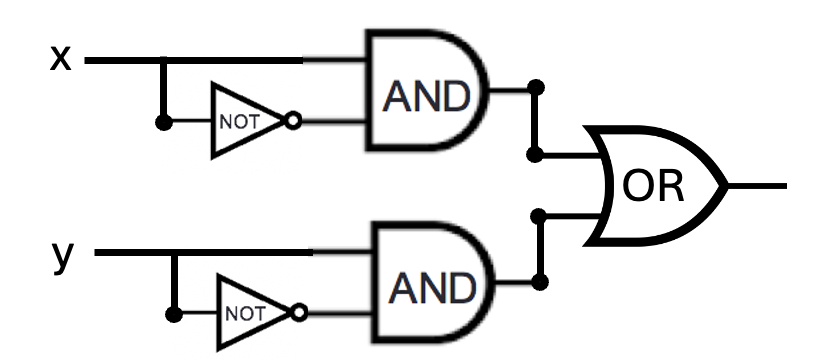
\includegraphics[width=2in]{../../files/circuits-hw3.png}
        \end{center}

        \item\gradeCorrect  Is there a way to fill in the blank portion of 
        the two logic circuits below *with the same gates connected in the same way*
        so that the resulting circuits have the same 
        input-output value *even though* one uses an OR gate at the end and the other 
        uses an XOR gate? If so, design the circuit that would be used, write 
        out the input-output table that results, and briefly explain why your 
        design works. If not, explain why not with reference to the definitions
        of the logic gates.
        \begin{multicols}{2}
            \begin{center}
                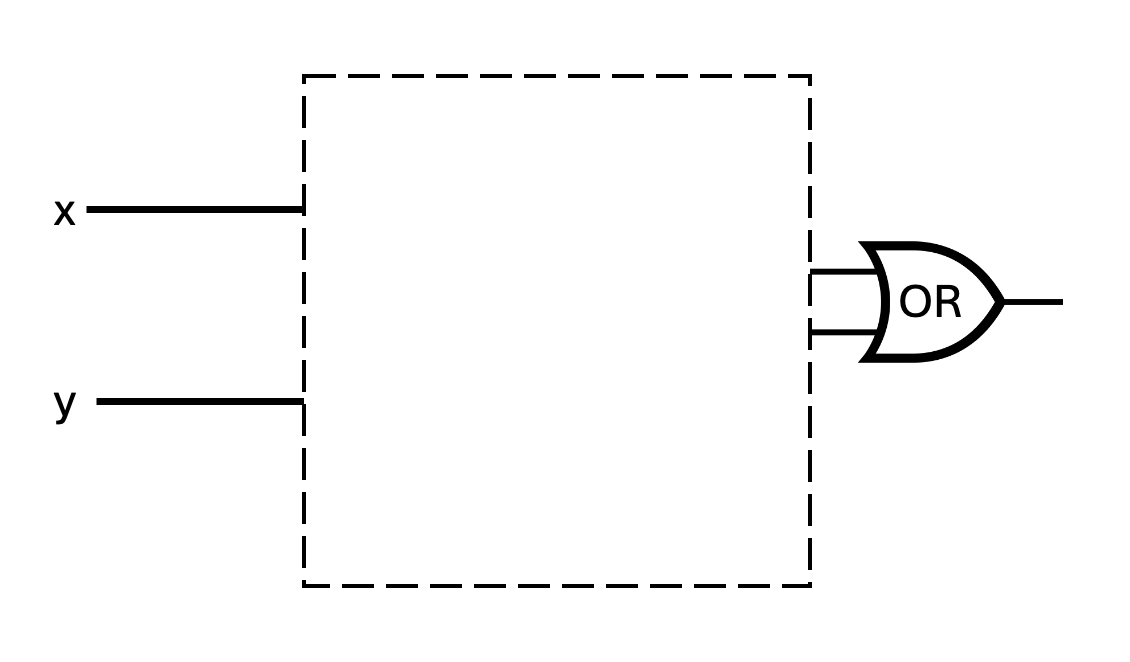
\includegraphics[width=2in]{../../files/circuit-blank-or-hw3.png}
            \end{center}
     
            \begin{center}
                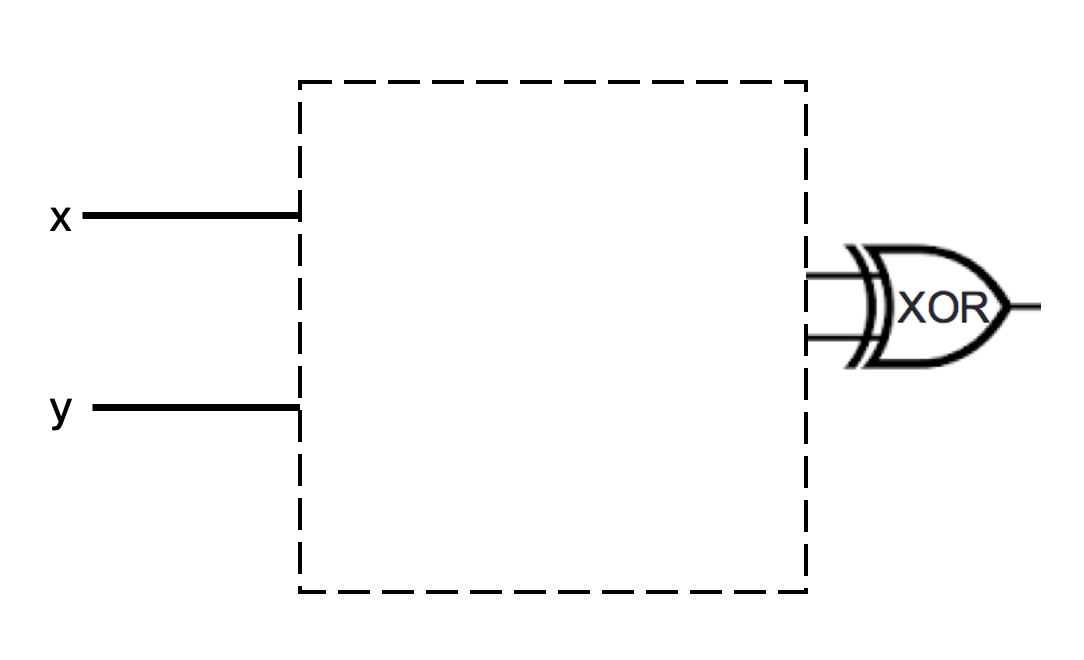
\includegraphics[width=2in]{../../files/circuit-blank-xor-hw3.png}
            \end{center}
        \end{multicols}

    \end{enumerate}
    \newpage
    \item Compound propositions. The set of strings of length $4$ whose characters are $0$s or $1$s is
        the result of four successive set-wise concatenations: $\{0,1\} \circ \{0,1\} \circ \{0,1\}\circ \{0,1\}$. Let's call
        this set $X_4$. Consider the function $f: X_4 \to X_4$ defined by
        $$ f(x) = 
        \begin{cases} 
            y &\text{when $(x)_{2,4} < 15$ and $(y)_{2,4} = (x)_{2,4} + 1$}\\
            1111 &\text{when $x = 1111$}
        \end{cases}$$
        for each $x \in X_4$. In other words, we can describe the function as: $f$ takes a string, interprets it as the binary fixed-width $4$
        expansion of an integer, and then adds $1$ to that integer (unless $x$ is already representing
        the greatest integer that can be represented in binary fixed-width $4$) and outputs the binary 
        fixed-width $4$ expansion of the result.
        \begin{enumerate} 
        \item\gradeComplete Fill in the blanks in the following input-output definition table 
        with four inputs $x_3$, $x_2$, $x_1$, $x_0$ and four outputs $y_3$, $y_2$, $y_1$, $y_0$
        so that $f(x_3x_2x_1x_0) = y_3y_2y_1y_0$.
        
        \begin{center}
        \begin{tabular}{cccc|cccc}
        $x_3$ & $x_2$ & $x_1$ & $x_0$ & $y_3$ & $y_2$ & $y_1$ & $y_0$\\
        \hline
        $1$ & $1$ & $1$ & $1$ & $1$ & $1$ & BLANK1 & $1$\\
        $1$ & $1$ & $1$ & $0$ & $1$ & $1$ & $1$ & $1$\\
        $1$ & $1$ & $0$ & $1$ & $1$ & BLANK2 & $1$ & $0$\\
        $1$ & $1$ & $0$ & $0$ & $1$ & $1$ & $0$ & $1$\\
        $1$ & $0$ & $1$ & $1$ & $1$ & $1$ & $0$ & $0$\\
        $1$ & $0$ & $1$ & $0$ & $1$ & $0$ & $1$ & $1$\\
        $1$ & $0$ & $0$ & $1$ & $1$ & $0$ & $1$ & $0$\\
        $1$ & $0$ & $0$ & $0$ & BLANK3& $0$ & $0$ & $1$\\
        $0$ & $1$ & $1$ & $1$ & $1$ & $0$ & $0$ & $0$\\
        $0$ & $1$ & $1$ & $0$ & $0$ & $1$ & $1$ & BLANK4\\
        $0$ & $1$ & $0$ & $1$ & $0$ & $1$ & $1$ & BLANK5\\
        $0$ & $1$ & $0$ & $0$ & $0$ & $1$ & $0$ & $1$\\
        $0$ & $0$ & $1$ & $1$ & $0$ & $1$ & $0$ & $0$\\
        $0$ & $0$ & $1$ & $0$ & $0$ & $0$ & $1$ & $1$\\
        $0$ & $0$ & $0$ & $1$ & $0$ & $0$ & $1$ & $0$\\
        $0$ & $0$ & $0$ & $0$ & BLANK6 & $0$ & $0$ & $1$\\
        \end{tabular}
        \end{center}
  
        \item\gradeCorrect
        Construct an expression (as a compound proposition) for $y_0$ in terms of the inputs 
        $x_3, x_2, x_1, x_0$. Justify your expression by referring to the definition of the logic 
        gates XOR, AND, OR, NOT and the definition of the function $f$. Hint: our work on the half-adder might 
        be helpful.
        \item\gradeCorrect
        Construct an expression (as a compound proposition) for $y_1$ in terms of the inputs 
        $x_3, x_2, x_1, x_0$. Justify your expression by referring to the definition of the logic 
        gates XOR, AND, OR, NOT and the definition of the function $f$. Hint: our work on the half-adder might 
        be helpful.
        \item\gradeComplete Draw a combinatorial circuit corresponding to these compound propositions.
        Remember that the symbols for the inputs will be on the left-hand-side and 
        the symbol for the outputs $y_0$ and $y_1$ will be on the right-hand side. Use gates (draw the appropriate
        shapes and add labels for clarity) and wires to connect the inputs appropriately to give the output.
        \item\gradeComplete Construct expressions (as a compound propositions) for $y_2$ and $y_3$ 
        in terms of the inputs  $x_3, x_2, x_1, x_0$. Are these similar to the expressions for $y_0$ and $y_1$?
        \end{enumerate}
        \item Logical Equivalence. Imagine a friend suggests the following argument to you: ``The compound proposition
        \[
        (x \lor y) \land z
        \]
        is logically equivalent to 
        \[
        x \lor (y \land z)
        \]
        because I can transform one to the other using the following sequence of logical equivalences: 
        \[
           (x \lor y) \land z \equiv
           (x \lor (y \land y)) \land z \equiv
           x \lor ( (y \lor y) \land z) \equiv x \lor (y \land z) 
        \]
        because $y$ is logically equivalent to both $y \land y$ and to $y \lor y$".
        
        \begin{enumerate}
        \item\gradeCorrect Prove to your friend that they made a mistake by giving a truth
        assignment to the propositional variables $x,y,z$ so that 
        the two compound propositions 
        $ (x \lor y) \land z$ and $ x \lor (y \land z)$ have different truth values.
        Justify your choice by evaluating these compound propositions using the definitions of the logical connectives 
        and include enough intermediate steps so that a student in CSE 20 who may be 
        struggling with the material can still follow along with your reasoning.
        
        \item\gradeComplete 
        Help your friend find the problem in their argument by pointing out which step(s) were incorrect.
        
        \item\gradeComplete Give {\bf three} different compound propositions
        that are actually logically equivalent to (and not the same as)
        \[
            (x \lor y) \land z
        \]
        Justify each one of these logical equivalences either by applying a sequence of logical equivalences
        or using a truth table.  Notice that you can use other logical operators (e.g. $\lnot, \lor, \land, \oplus, \to, 
        \leftrightarrow$) 
        when constructing your compound propositions.
     
        {\it Bonus; not for credit (do not hand in)}: How would you translate each of the equivalent compound
        propositions in English? Does doing so help illustrate why they are equivalent?
        \end{enumerate}
        
     
\end{enumerate}

\newpage


\title{hw4-proofs-and-sets}
\date{Due: 5/14/24 at 5pm (no penalty late submission until 8am next morning)}

\maketitle
\thispagestyle{fancy}


{\bf In this assignment}, you will use propositional and predicate logic to evaluate
statements and arguments. You will analyze statements and determine if they are true or false using valid proof strategies.
You will also determine if candidate arguments are valid.


{\bf Relevant class material}: Weeks 4,5,6.

You will submit this assignment via Gradescope
(\href{https://www.gradescope.com}{https://www.gradescope.com}) 
in the assignment called ``hw4-proofs-and-sets''.

\instructions


\vspace{-10pt}

In your proofs and disproofs of statements below, justify each  step
by reference to  a component of the  following proof  strategies
we  have discussed so far, and/or to relevant definitions and calculations.

\vspace{-10pt}

\begin{itemize}
    \item A counterexample can be used to prove that  $\forall x P(x)$ is {\bf false}.
    \item  A witness can be used  to  prove that  $\exists x P(x)$ is {\bf true}.
    \item {\bf Proof of universal by exhaustion}: To prove that $\forall x \, P(x)$
is true when $P$ has a finite domain, evaluate the predicate at {\bf each} domain element to confirm that it is always T.
    \item  {\bf Proof by universal generalization}: To prove that $\forall x \, P(x)$
is true, we can take an arbitrary element $e$ from the domain and show that $P(e)$ is true, without making any assumptions about $e$ other than that it comes from the domain.
    \item To  prove  that $\exists x P(x)$ is {\bf false}, write the universal statement that is logically equivalent to its negation and then prove it true using universal generalization.
    \item {\bf Strategies for conjunction}: To prove that $p \land q$ is true, have two subgoals: subgoal (1) prove $p$ 
is  true; and, subgoal (2) prove $q$ is true. To prove that $p \land q$ is false, it's enough to prove that $p$ is false.
 To prove that $p \land q$ is false, it's enough to prove that $q$ is false.
    \item {\bf Proof of Conditional by Direct Proof}: To prove that the implication $p \to q$ is true, we can assume $p$ is true and use that assumption to show $q$ is true.
    \item {\bf Proof of Conditional by Contrapositive Proof}: To prove that the implication $p \to q$ is true, we can assume $\neg q$ is true and use that assumption to show $\neg p$ is true.
    \item {\bf Proof by Cases}: To prove $q$ when we know $p_1 \lor p_2$, show that $p_1 \to q$ and $p_2 \to q$.
\end{itemize}


{\bf Assigned questions}

\begin{enumerate}[labelindent=0pt, leftmargin=0pt]
    \item  Evaluating predicates. Consider the following predicates, each of which has 
    as its domain the set of all bitstrings whose leftmost bit is $1$
    
    $E(x)$ is $T$ exactly when $(x)_{2}$ is even, and is $F$ otherwise
    
    $L(x)$ is $T$ exactly when $(x)_2 < 15$, and is $F$ otherwise
    
    $M(x)$ is $T$ exactly when $(x)_2 > 2$ and is $F$ otherwise.
    
    
    \rule{0.5\textwidth}{.4pt}
    
    {\it Sample response that can be used as reference for the detail expected 
    in your answer:} To prove that the statement $$\forall x ~L(x)$$ is false, we can use 
    the counterexample $x = 1111$, which is a bitstring whose leftmost bit is $1$ (so is in the domain).
    Applying the definition of $L(x)$, since $(1111)_2 = 1 \cdot 2^3 + 1\cdot 2^2 + 1 \cdot 2^1 + 1 \cdot 2^0 = 8 + 4+2+1 = 15$
    which is not (strictly) less than $15$, we have that $L(1111) = F$ and so the universal statement is false.
    
    
    \rule{0.5\textwidth}{.4pt}
    
    
    
    \begin{enumerate}
    \item\gradeCorrectFirst Use a counterexample to prove that the statement
    \[
    \forall x ( ~L(x) \to E(x)~)
    \]
    is false.
    
    \item\gradeCorrect Use a witness to prove that the statement
    \[
    \exists x (~L(x) \land M(x) ~)
    \]
    is true.
    
    \item\gradeCompleteFirst Translate each of the statements in the previous two
    parts to English.
    \end{enumerate}


    \item Set properties. Let $W = \mathcal{P}(\{1,2,3,4,5\})$. 


    \rule{0.5\textwidth}{.4pt}
    
    {\it Sample response that can be used as reference for the detail expected 
    in your answer for parts (a) and (b) below:} 
    
    To give an example element in the set 
    $\{ X \in W ~|~ 1 \in X \} \cap \{ X \in W ~|~  2 \in X \}$,
    consider $\{ 1,2\}$. To prove that this is in the set, by definition of intersection, we need to show
    that $\{1,2\} \in \{ X \in W ~|~ 1 \in X \}$ and that $\{1,2\} \in \{ X \in W ~|~ 2 \in X \}$.
    \begin{itemize}
    \item By set builder notation, elements in $\{ X \in W ~|~ 1 \in X \}$ have to be elements of $W$ which have $1$ as an element. By definition of power set, elements of $W$ are subsets of $\{1,2,3,4,5\}$. Since
    each element in $\{1,2\}$ is an element of $\{1,2,3,4,5\}$, $\{1,2\}$ is a subset of $\{1,2,3,4,5\}$ 
    and hence is an element of $W$. Also, by roster method, $1 \in \{1,2\}$. Thus, $\{1,2\}$ satisfies the 
    conditions for membership in $\{ X \in W ~|~ 1 \in X \}$.
    \item Similarly, by set builder notation, elements in $\{ X \in W ~|~ 2 \in X \}$ have to be elements of $W$ 
    which have $2$ as an element. 
    By definition of power set, elements of $W$ are subsets of $\{1,2,3,4,5\}$. Since
    each element in $\{1,2\}$ is an element of $\{1,2,3,4,5\}$, $\{1,2\}$ is a subset of $\{1,2,3,4,5\}$ 
    and hence is an element of $W$. Also, by roster method, $2 \in \{1,2\}$. Thus, $\{1,2\}$ satisfies the 
    conditions for membership in $\{ X \in W ~|~ 2 \in X \}$.
    \end{itemize}
    
    \rule{0.5\textwidth}{.4pt}
    
    
    \begin{enumerate}
    \item\gradeCorrect Give two (different) example elements in 
    \[
    W \times \mathcal{P}(W)
    \]
    Justify your examples by explanations that include references to the relevant definitions.
    
    \item\gradeCorrect Give one example element in 
    \[
    \{ X \in W \mid (1 \in X) \land (X \cap \{3,4\} = \emptyset) \}
    \]
    Justify your example by explanations that include references to the relevant definitions.
    
    \item\gradeComplete Consider the following statement and attempted proof:
    
    
    $$\forall A \in W \, \forall B \in W ~\left(~((A \cap B) \subseteq A) \to (A \subseteq B)~\right)$$
    
    \begin{quote}
    (1) Towards a universal generalization argument, {\bf choose arbitrary} $A \in W, B \in W$ .
    
    (2) We need {\bf to show} $((A \cap B) \subseteq A) \to (A \subseteq B)$.
    
    (3) Towards a proof of the conditional by the contrapositive, {\bf assume} $A \subseteq B$, and we need {\bf to show} 
    that $(A \cap B) \subseteq A$.
    
    (4) By definition of subset inclusion, this means we need {\bf to show} 
    $\forall x ~( x \in A \cap B \to  x \in A  ~)$.
    
    (5) Towards a universal generalization, {\bf choose arbitrary} $x$; we need {\bf to show} that \\
    $x \in A \cap B \to x \in A$.
    
    (6) Towards a direct proof, {\bf assume} $x \in A \cap B$, and we need {\bf to show } $x \in A$.
    
    (7) By definition of set intersection and set builder notation, we have that $x \in A \land x \in B$.
    
    (8) By the definition of conjunction, $x \in A$, which is  what we needed to show. QED
    \end{quote}
    
    Demonstrate that this attempted proof is invalid by providing
    and justifying a {\bf counterexample} (disproving the statement).
    Then, explain why this attempted proof is 
    invalid by identifying in which step a definition or proof strategy is used incorrectly, and describing how the 
    definition or proof strategy was misused.

    \item \gradeComplete A Venn diagram is a chart of overlapping regions that illustrates the similarities
    differences of a collection of sets. You may have seen some examples in memes, including
    these (from a web search):
    \begin{center}
        \hfill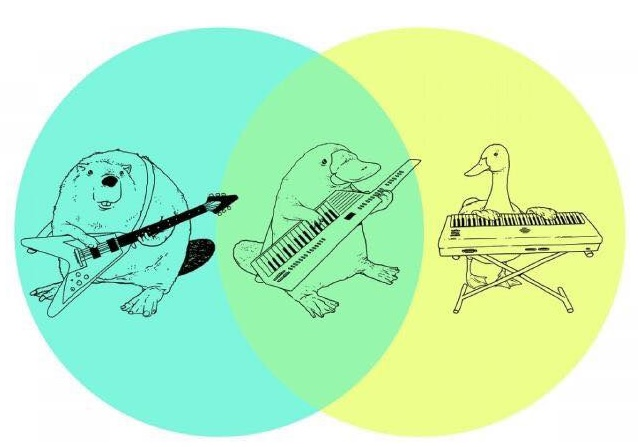
\includegraphics[width=1.5in]{../../resources/images/funny-pictures-venn-diagram-duck-5448120.jpeg} \hfill
        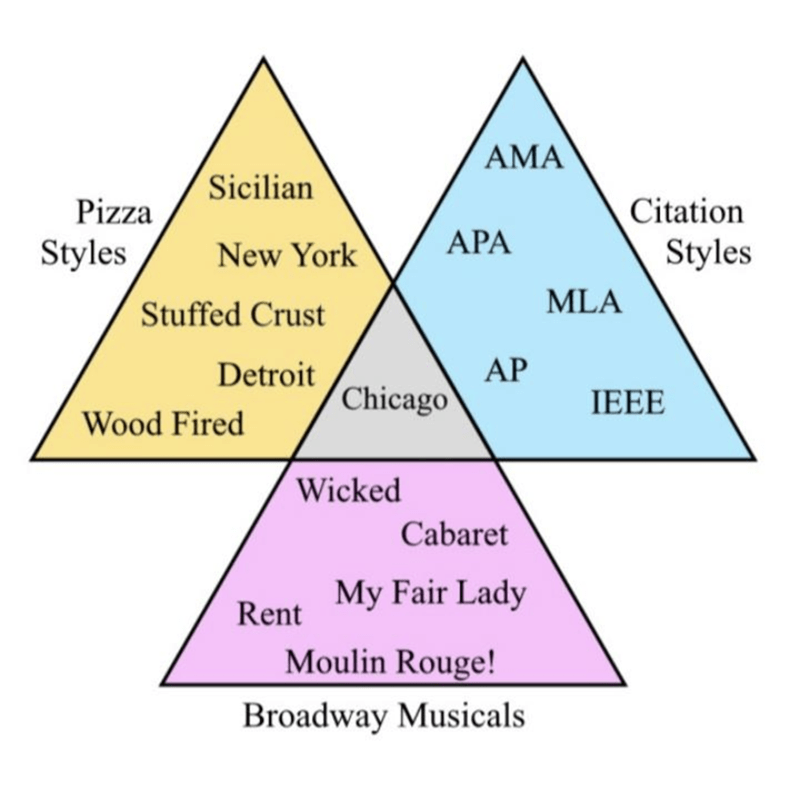
\includegraphics[width=1.5in]{../../resources/images/detroit-ap-chicago-ieee-wood-fired-wicked-cabaret-my-fair-lady-rent-moulin-rouge-broadway-musicals.png}
        \hfill
    \end{center}
    Mostly we see Venn Diagrams with 2 or 3 circles (or other shapes). In this question, 
    we consider how to draw a Venn Diagram with 4 regions.
    \begin{enumerate}
        \item Here is a Venn Diagram with 2 circles. Each region is labelled (encoded) with a 
        binary string with 2 bits. Notice that there are four regions: the region outside
        of the two circles, the region inside the left circle and not the right circle, the region 
        inside the right circle and not the left circle, and the region inside both circles.
        \begin{center}
            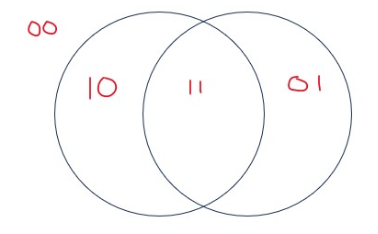
\includegraphics[width=1.5in]{../../resources/images/VennDiagram2Circles.png}
        \end{center}
        Generalize this encoding by encoding each region in this 3 circle Venn Diagram with 
        a unique binary string with 3 bits.
        \begin{center}
            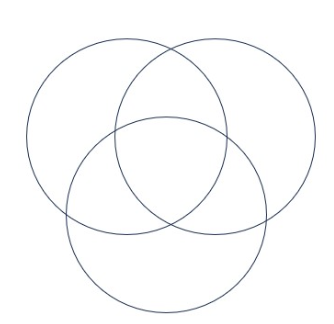
\includegraphics[width=1.5in]{../../resources/images/VennDiagram3Circles.png}
        \end{center}
        \item Give an alternate representation of the regions in the 2 circle and 3 circle 
        Venn Diagrams by labelling each circle with a letter ($X$, $Y$, $Z$, or $A$, $B$, $C$, for 
        example) and then expressing each region as the result of combining these with set operations
        (like union, intersection, and set difference).
        \item Here are two attempts at a Venn Diagram with 4 shapes, one with circles and the other 
        with ellipses.
        \begin{center}
            \hfill
            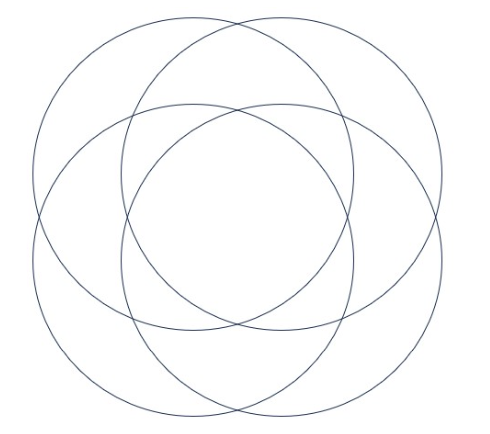
\includegraphics[width=1.5in]{../../resources/images/VennDiagram4Circles.png}
            \hfill 
            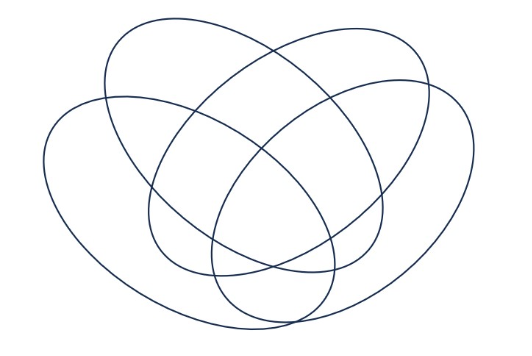
\includegraphics[width=1.5in]{../../resources/images/VennDiagram4Ellipses.png}
            \hfill
        \end{center}
        Is there anything missing from either diagram? (How many regions are there? 
        How many regions should there be in order to use each 4 bit binary string 
        exactly once in a generalization of the encoding we saw before?) 
        If you had to choose one of these diagrams, which would you choose, and why?
    \end{enumerate}
    (This question is adapted from one created by Miles Jones and is used with permission.)
    \end{enumerate}
    
    
    \item Number properties. Consider the predicate  $F(~(a,b)~)  = ``a \text{ is a factor of } b"$ 
    over  the domain $\mathbb{Z}^{\neq 0} \times \mathbb{Z}$. Consider the following quantified
    statements
    \begin{multicols}{2}
    \begin{enumerate}[label=(\roman*)]
    \item $\forall x \in \mathbb{Z} ~(F(~(1,x~)))$
    \item $\forall x \in \mathbb{Z}^{\neq 0} ~(F(~(x,1)~))$
    \item $\exists x \in \mathbb{Z} ~(F(~(1,x)~))$
    \item $\exists x \in \mathbb{Z}^{\neq 0} ~(F(~(x,1)~))$
    \item $\forall x \in \mathbb{Z}^{\neq 0} ~\exists y \in \mathbb{Z} ~(F(~(x,y)~))$
    \item $\exists x \in \mathbb{Z}^{\neq 0} ~\forall y \in \mathbb{Z} ~(F(~(x,y)~))$
    \item $\forall y \in \mathbb{Z} ~\exists x \in \mathbb{Z}^{\neq 0} ~(F(~(x,y)~))$
    \item $\exists y \in \mathbb{Z} ~\forall x \in \mathbb{Z}^{\neq 0} ~(F(~(x,y)~))$
    \end{enumerate}
    \end{multicols}
    
    \begin{enumerate}
    
    \item\gradeComplete
    Which of the statements (i) - (viii) is being {\bf proved} by the following proof:
    
    \begin{quote}
      By universal generalization, {\bf choose} $e$ to be an {\bf arbitrary} integer. 
      We need to show that $F(~(1,e)~)$. By definition of the  predicate $F$, we can rewrite 
      this goal as $\exists c \in \mathbb{Z}~(e = c \cdot 1)$. We pick the {\bf witness} $c = e$, 
      which is an integer and therefore in the domain. Calculating, 
      $c \cdot 1 = e \cdot 1 = e$, as required. Since the predicate $F(1,e)$ evaluates to true 
      for the arbitrary integer $e$, the claim has been proved. $\square$
    \end{quote}
    
    
    {\it Hint: it may be useful to 
    identify the key words in the proof that indicate proof strategies.}
    
    \item\gradeComplete
    Which of the statements (i) - (viii) is being {\bf disproved} by the following proof:
    
    \begin{quote}
      To disprove the statement, we need to find a counterexample. We choose $2$, a nonzero
      integer so in the domain. We need to show that $\lnot F(~(2,1)~)$. By definition of the predicate $F$, we 
      can rewrite this goal as $1 \textbf{ mod } 2 \neq 0$. By definition of integer division, since 
      $1 = 0 \cdot 2  + 1$ (and $0 \leq 1 < 2$), $1 \textbf { mod } 2 = 1$ which is nonzero so the counterexample works to 
      disprove the original statement.
       $\square$
    \end{quote}
    
    {\it Hint: it may be useful to 
    identify the key words in the proof that indicate proof strategies.}
    
    \item ({\it Graded for correctness of evaluation of statement (is it true or false?) and fair effort completeness of the translation and proof}) 
    Translate the statement to English, state whether is it true or false, and then justify your answer (by proving the statement or its negation).
    $$\exists x \in \mathbb{Z}^{\neq 0}~ \exists y \in \mathbb{Z}^{\neq 0} ~(~\lnot(x = y) \land F(~(x,y)~) \land F(~(y,x)~)~)$$
    
    \item ({\it Graded for correctness of evaluation of statement (is it true or false?) 
    and fair effort completeness of the translation and of the proof}) 
    Translate the statement to English, state whether is it true or false, and then justify your answer (by proving the statement or its negation).
    $$\forall x \in \mathbb{Z}^{\neq 0}~ \forall y \in \mathbb{Z}^{\neq 0} ~(~F(~(x,y)~) \to \lnot F(~(y,x)~)~)$$
    
    \item ({\it Graded for correctness of evaluation of statement (is it true or false?) 
    and fair effort completeness of the translation and of the proof}) 
    Translate the statement to English, state whether is it true or false, and then justify your answer (by proving the statement or its negation).
    $$\exists x \in \mathbb{Z}^{\neq 0}~ \exists y \in \mathbb{Z}~(~F(~(x,y)~) \land  F(~(x+1, y)~) \land F(~(x+2, y)~)~)$$
    
    \item ({\it Graded for correctness of evaluation of statement (is it true or false?) 
    and fair effort completeness of the translation and of the proof}) 
    Translate the statement to English, state whether is it true or false, and then justify your answer (by proving the statement or its negation).
    $$\forall x \in \mathbb{Z}^{\neq 0}~ (~F(~(x,x^2)~) \land F(~(x,x^3)~)~)$$
    
    \end{enumerate}
    
    \item Structural induction. Recall that we define the set of bases as $B  =  \{ \A, \C, \U, \G \}$.
The set of RNA strands $S$ is defined (recursively) by:
\[
\begin{array}{ll}
\textrm{Basis Step: } & \A \in S, \C \in S, \U \in S, \G \in S \\
\textrm{Recursive Step: } & \textrm{If } s \in S\textrm{ and }b \in B \textrm{, then }sb \in S
\end{array}
\]
where $sb$ is string concatenation. 
The function \textit{rnalen} that computes the length of RNA strands in $S$ is defined recursively by
$rnalen: S  \to \mathbb{Z}^+$


\begin{quote}
Basis step: If $b \in B$ then $rnalen(b)  = 1$

Recursive step: If $s \in S$ and $b \in B$, then $rnalen(sb)  = 1 + rnalen(s)$
\end{quote}

The function \textit{basecount} that computes the number of a given base 
$b$ appearing in a RNA strand $s$ is defined recursively:
    
\[
\begin{array}{llll}
& & \textit{basecount} : S \times B & \to \mathbb{N} \\
\textrm{Basis Step:} &  \textrm{If } b_1 \in B, b_2 \in B & \textit{basecount}(~(b_1, b_2)~) & =
        \begin{cases}
            1 & \textrm{when } b_1 = b_2 \\
            0 & \textrm{when } b_1 \neq b_2 \\
        \end{cases} \\
\textrm{Recursive Step:} & \textrm{If } s \in S, b_1 \in B, b_2 \in B &\textit{basecount}(~(s b_1, b_2)~) & =
        \begin{cases}
            1 + \textit{basecount}(~(s, b_2)~) & \textrm{when } b_1 = b_2 \\
            \textit{basecount}(~(s, b_2)~) & \textrm{when } b_1 \neq b_2 \\
        \end{cases}
\end{array}
\]
\begin{enumerate}
\item ({\it Graded for correctness of evaluation of statement (is it true or false?) and fair effort completeness of the translation and proof}) 
Translate the statement to English, state whether is it true or false, and then justify your answer (by proving the statement or its negation).
$$\forall b \in B ~\exists s \in S ~(~rnalen(s) = basecount(~(s,b)~)~)$$

\item ({\it Graded for correctness of evaluation of statement (is it true or false?) 
and fair effort completeness of the translation and of the proof}) 
Translate the statement to English, state whether is it true or false, and then justify your answer (by proving the statement or its negation).
$$\forall s \in S~ (rnalen(s) > basecount( ~(s,\A)~))$$

\item ({\it Graded for correctness of evaluation of statement (is it true or false?) 
and fair effort completeness of the translation and of the proof}) 
Translate the statement to English, state whether is it true or false, and then justify your answer (by proving the statement or its negation).
$$\forall s \in S~ \forall b \in B ~( basecount( ~(s,b)~) > 0)$$

\end{enumerate}

\end{enumerate}

\newpage

\title{hw5-proofs-and-induction}
\date{Due: 5/21/24 at 5pm (no penalty late submission until 8am next morning)}

\maketitle
\thispagestyle{fancy}

{\bf In this assignment}, you will work with recursively defined sets and functions and prove 
properties about them, practicing induction and other proof strategies.

{\bf Relevant class material}: Weeks 5,6,7.

You will submit this assignment via Gradescope
(\href{https://www.gradescope.com}{https://www.gradescope.com}) 
in the assignment called ``hw5-proofs-and-induction''.

\instructions

In your proofs and disproofs of statements below, justify each  step
by reference to  a component of the  following proof  strategies
we  have discussed so far, and/or to relevant definitions and calculations.

\vspace{-10pt}

\begin{itemize}
    \item A counterexample can be used to prove that  $\forall x P(x)$ is {\bf false}.
    \item  A witness can be used  to  prove that  $\exists x P(x)$ is {\bf true}.
    \item {\bf Proof of universal by exhaustion}: To prove that $\forall x \, P(x)$
is true when $P$ has a finite domain, evaluate the predicate at {\bf each} domain element to confirm that it is always T.
    \item  {\bf Proof by universal generalization}: To prove that $\forall x \, P(x)$
is true, we can take an arbitrary element $e$ from the domain and show that $P(e)$ is true, without making any assumptions about $e$ other than that it comes from the domain.
    \item To  prove  that $\exists x P(x)$ is {\bf false}, write the universal statement that is logically equivalent to its negation and then prove it true using universal generalization.
    \item {\bf Strategies for conjunction}: To prove that $p \land q$ is true, have two subgoals: subgoal (1) prove $p$ 
is  true; and, subgoal (2) prove $q$ is true. To prove that $p \land q$ is false, it's enough to prove that $p$ is false.
 To prove that $p \land q$ is false, it's enough to prove that $q$ is false.
    \item {\bf Proof of Conditional by Direct Proof}: To prove that the implication $p \to q$ is true, we can assume $p$ is true and use that assumption to show $q$ is true.
    \item {\bf Proof of Conditional by Contrapositive Proof}: To prove that the implication $p \to q$ is true, we can assume $\neg q$ is true and use that assumption to show $\neg p$ is true.
    \item {\bf Proof by Cases}: To prove $q$ when we know $p_1 \lor p_2$, show that $p_1 \to q$ and $p_2 \to q$.
    \item
    {\bf Proof by Structural Induction}: To prove that $\forall x \in X \, P(x)$ where $X$ is a recursively defined set, prove two cases:
        
        \begin{tabularx}{\textwidth}{l X}
        Basis Step: & Show the statement holds for elements specified in the basis step of the definition. \\
        Recursive Step: & Show that if the statement is true for each of the elements used to construct
    new elements in the recursive step of the definition, the result holds for these new elements.
    \end{tabularx}
    
    \item {\bf Proof by Mathematical Induction}: To prove a universal quantification over the set of  all integers greater than  or  equal to some base integer $b$:
    
    \begin{tabularx}{\textwidth}{l X}
        Basis Step: & Show the statement holds for $b$. \\
        Recursive Step: & Consider an arbitrary integer $n$ greater than or  equal to  $b$, assume
        (as the {\bf induction hypothesis})  that the property holds  for $n$, and use  this and
        other facts to  prove that  the property holds for $n+1$.
    \end{tabularx}
    
    \item {\bf Proof by Strong Induction} To prove that a universal quantification over the set of all integers greater than or equal to some  base integer $b$ holds,  pick a  fixed nonnegative integer  $j$ and then: \hfill 
    
    \begin{tabularx}{\textwidth}{l X}
        Basis Step: & Show the statement holds for $b$, $b+1$, \ldots, $b+j$. \\
        Recursive Step: & Consider an arbitrary integer $n$ greater than or  equal to  $b+j$, assume
        (as the {\bf strong  induction hypothesis})  that the property holds  for {\bf each of} $b$, $b+1$, \ldots, $n$, 	
        and use  this and
        other facts to  prove that  the property holds for $n+1$.
    \end{tabularx}

    \item {\bf Proof by Contradiction} 

    To prove that a statement $p$ is true, pick another statement $r$ and once we show
    that $\neg p  \to (r \wedge  \neg r)$ then  we can conclude that  $p$ is  true.
    
    {\it Informally} The statement we care about can't possibly be false, so it must be true.
\end{itemize}


{\bf Assigned questions}

\begin{enumerate}[labelindent=0pt, leftmargin=0pt]
    \item Mathematical and strong induction for properties of numbers.

    \begin{enumerate}
    \item \gradeCompleteFirst    Consider each of the following statements and attempted proofs below. Pretend you are the TA/tutor for CSE 20 and grade each of these attempts. 
    In particular, you should give each one a score out of $5$ points and justify your decisions with {\bf specific}, 
    {\bf actionable}, and {\bf justified} feedback;
    your explanations should be convincing but brief.
    Here is the rubric\footnote{According to the Merriam Webster definition, a {\bf rubric} is ``a guide listing specific criteria for grading or scoring academic papers, projects, or tests''. For CSE 20, you can see the rubrics 
    we use to grade assignments and exams on Gradescope: next to your submission for each question you will
    find the rubric items and associated point values. The highlighted items are the ones we select
    to describe your work; these correspond to the score assigned for the question.} you should use: 
    \begin{description}
    \item[5 points] Induction proof includes correctly executed base case
     and recursive step (with induction hypothesis, IH, clearly and correctly defined and used). Uses clear and correct calculations and references to definitions in both steps, including using the IH, to conclude both.
    \item[4 points] Induction proof includes base case and recursive step (with induction hypothesis clearly and mostly correctly defined and used),
    where base case attempted but incomplete OR, incorrect base element chosen but valid proof made for chosen
    element, OR induction hypothesis incorrectly stated but correctly used.
    \item[3 points] Any one of the following: (1) Induction proof with correctly executed base case 
    and recursive step that demonstrates
    connection between induction hypothesis and property being true for $n+1$, some missing or 
    incorrect logical glue; (2) Induction proof with missing base case and correctly executed recursive step.
    \item[2 points] Any one of the following: (1) Induction proof includes attempts at correct steps of an 
    induction proof (base case, recursive  step), with significant logical gaps and/or errors; (2) correctly executed base case 
    with missing / incorrect recursive step,
    \item[1 point] Demonstrates knowledge of proof techniques (e.g.\ attempts some proof type other than 
    induction, but uses some proof technique correctly) and/or structure of induction argument.
    \end{description}
    
    \begin{enumerate}
\item Statement: ``the sum of the first 
$n$ positive odd integers is $n^2$"

{\bf Attempted Proof: }
\begin{quote}

Base Case: $n = 1$\\
First odd number is $1$; $1^2 = 1$. True.\\
$(n + 1)^2 = n^2 + 2n + 1$\\
$n^2$ is the sum of the first $n$ odd numbers, and $2n + 1$ is the next odd number in the sequence, therefore $(n + 1)^2 =$ the sum of the first $n + 1$ odd numbers.
\end{quote}


\item Statement: ``For every nonnegative integer $n$, $3 | n$." (Recall that the $\mid$ symbol is used to mean ``divides'' or ``is a factor of''.)

{\bf Attempted Proof: }
  \begin{quote}
   Attempted Proof: We proceed by strong mathematical induction.

{\it Basis step:} Indeed, $3 | 0$ because there is an integer, namely $0$ such that $0 = 3\cdot 0$.


{\it Induction step:} Let $k$ be arbitrary.  Assume, as the strong induction hypothesis, 
    that for all nonnegative integers $j$ with $0 \leq j \leq k$, that $3 | j$.  Write $k+1 = m + n$, where
    $m,n$ are integers less than $k+1$.  By the induction hypothesis, $3 | m$ and $3 | n$.  That is, there
    are integers $a,b$ such that $m = 3a$ and $n=3b$.  Therefore, $k+1 = (3a) + (3b) = 3 (a+b)$.
    We can choose $a + b$, where we know $a + b \in \mathbb{Z}$, to show that $3 | (k+1)$, as
     required.
     \end{quote}

    \end{enumerate}

    \item \gradeComplete Decide whether each statement above is true or false, 
    give correct and complete induction proofs for the true statement(s) and disprove 
    by counterexample for the false statement(s).
    \end{enumerate}

    \item \gradeCorrect Games and induction.  The game of Nim-Var is a two-player game (which is a variant of Nim).
    At the start of the game, there are two piles, each containing $n$ 
    jelly beans
    ($n$ is a positive integer).  On a player's turn, that player picks one 
    of the two piles and does {\bf one} of the following: either
    \begin{itemize}
    \item removes some positive number of jelly beans from that pile, {\bf or}
    \item moves some positive number of jelly beans (that is less than the
    current total number of jelly beans in the pile) from that pile to the other.  
    {\it Note: if there is only one jelly bean left in a pile, the player cannot move
    this jelly bean to the other pile.}
    \end{itemize}
    The player to take the last jelly bean wins.  
    Use strong induction to prove that the second player always has a winning strategy in Nim-Move.
    A complete and correct solution will first identify what the strategy is, and then prove that 
    following this strategy will lead the second player to win the game (no matter what the first 
    player chooses to do at each turn).
    
    
    
    \item Linked Lists. Recall the recursive definition of the set of linked lists of 
    natural numbers (from class)
    \[
    \begin{array}{ll}
        \textrm{Basis Step: } & [] \in L \\
        \textrm{Recursive Step: } & \textrm{If } l \in L\textrm{ and }n \in \mathbb{N} \textrm{, then } (n, l) \in L
    \end{array}
    \]
    and the definitions of the function which gives the length of a linked list of natural numbers 
    $length: L \to \mathbb{N}$
        \[
        \begin{array}{llll}
            \textrm{Basis Step:} &  & length(~[]~) &= 0 \\
            \textrm{Recursive Step:} & \textrm{If } l \in L\textrm{ and }n \in \mathbb{N}\textrm{, then  } & length(~(n, l)~)  &= 1+ length(l)
        \end{array}
    \]
    the function $append : L \times \mathbb{N} \to L$ that 
    adds an element at the end of a linked list
    \[
        \begin{array}{llll}
        \textrm{Basis Step:} & \textrm{If } m \in \mathbb{N}\textrm{ then } & append(~([], m)~) & = (m, [])\\
        \textrm{Recursive Step:} & \textrm{If } l \in L\textrm{ and }n \in \mathbb{N}\textrm{ and }m \in \mathbb{N}\textrm{, then  } & append(~(~(n, l), m~)~)  &= (n, append(~(l, m)~)~)
        \end{array}
    \]
    and the function $prepend : L \times \mathbb{N} \to L$ that adds an element at the 
    front of a linked list 
    \[
    prepend(~(l, n)~) = (n, l)
    \]

    \rule{0.5\textwidth}{.4pt}
    
    {\it Sample response that can be used as reference for the detail expected 
    in your answer:} 
    To evaluate the result of $length(~(4,(2,(7,[])))~)$ we calculate: 
    \begin{align*}
        length(~(4,(2,(7,[])))~) &= 1 + length ( ~(2,(7,[]))~) \\
        & \qquad \qquad \text{using recursive step of definition of $length$, with $n=4, l=(2,(7,[]))$} \\
        &= 1 + 1 + length ( ~(7,[])~) \\
        & \qquad \qquad \text{using recursive step of definition of $length$, with $n=2, l=(7,[])$} \\
        &= 1 + 1 + 1+ length ( ~[]~) \\
        & \qquad \qquad \text{using recursive step of definition of $length$, with $n=7, l=[]$} \\
        &= 1 + 1 + 1 + 0\\
        & \qquad \qquad \text{using basis step of definition of $length$, since input to $length$ is $[]$} \\
    \end{align*}
    \rule{0.5\textwidth}{.4pt}
    

    In this question, we'll consider the combination of these functions with a new function, one 
    that removes the element at the front of the list (if there is any). We define $remove: L \to L$
    by
    \[
        \begin{array}{ll}
            \textrm{Basis Step: } & remove([]) = [] \\
            \textrm{Recursive Step: } & \textrm{If } l \in L\textrm{ and }n \in \mathbb{N} \textrm{, then } remove(~(n, l)~) = l
        \end{array}        
    \]
    \begin{enumerate}
        \item\gradeCorrect What is the result of $remove(~append(~(prepend~(~(~(10,[]), 5~)~), 20)~)~)$? 
        For full credit, include all intermediate steps with brief justifications for each.
        \item\gradeCorrect Prove the statement
        \[
            \forall l \in L \left(~ remove( prepend(~(l,0)~)) = l ~\right) 
        \]
        \item\gradeCorrect Disprove the statement
        \[
            \forall l \in L \left(~ remove( append(~(l,0)~)) = l ~\right) 
        \]
    \end{enumerate}

    \item Primes, divisors, and proof strategies. For each statement below, identify the {\bf main logical structure or connective} of the 
    statement, list the proof strategies that could be used to prove and to disprove a statement with that structure, 
    then identify whether the statement is true or false and justify with a proof of the statement or its negation. 
    ({\it Graded for correctness of identification of logical structure and proof strategies and evaluation of statement (is it true or false?) 
    and fair effort completeness of the proof}) 


    \rule{0.5\textwidth}{.4pt}
    
    {\it Sample response that can be used as reference for the detail expected 
    in your answer:} 

    Consider the statement: There is a greatest negative integer.

    The main logical structure for this statement is that it is an {\bf existential} statement, as we can 
    see by translating it to symbols: 
    \[
        \exists g \in \mathbb{Z}^{-} \forall x \in \mathbb{Z}^{-} ( g \geq x)
    \]
    To prove an existential statement, the main proof strategy we could use is to find a witness. 
    Proof by cases and proof by contradiction could also be used, because 
    both can be used to prove any statement (no matter its logical structure).

    To disprove an existential statement, we would need to prove its negation, which (using DeMorgan's Laws) can be 
    written as a universal statement. Therefore, to disprove this statement the strategies we could use are 
    universal generalization or structural induction (because $\mathbb{Z}^{-}$ is a recursively defined set) or 
    proof by cases or proof by contradiction. Notice that proof by exhaustion is not possible because the domain is not finite.

    The statement is true, as we can see from the witness $g = -1$, since it is in the domain $\mathbb{Z}^{-}$ and when we evaluate
    \[
        \forall x \in \mathbb{Z}^{-} ( -1 \geq x)
    \]
    we can proceed by universal generalization and take an arbitrary negative integer $x$, which by definition means $x < 0$, 
    and since $x$ is an integer, guarantees $x \leq -1 = g$, as required.
    \rule{0.5\textwidth}{.4pt}

        \begin{enumerate}
            \item The quotient of any even number with any nonzero even number is even.
            \item There are two odd numbers (not necessarily distinct) whose sum is even.
            \item The greatest common divisor of 5 and 23 is 1 and the greatest common divisior of 7 and 19 is 1.
            \item There are two positive integers greater than 20 that have the same greatest common divisor with 20. {\it Note: typo fixed, 
            originally said ``greatest common division'' instead of ``greatest common divisor''.}
        \end{enumerate}
    \end{enumerate}

\newpage

\setlength{\parindent}{0em}
\setlength{\parskip}{0em}

\title{Project}
\date{Due: 5/8/24 at 5pm (late submission until 8am next morning) - Extended by 24 hours}


\maketitle
\thispagestyle{fancy}

\vspace{-20pt}

In the project component of this class, you will extend your 
work on assignments and explore applications of your choosing. 
{\it Why?}
To go deeper and explore the material from discrete math and how it relates to Computer Science.
You will watch some videos and read some articles, and then connect them to our work in CSE 20. There 
are two tasks in the project, and for each one you will submit a short video and a PDF document, each 
addressing specific questions.


As you work on the project, keep in mind our three high-level goals for CSE 20:
\begin{itemize}
\item Model systems with tools from discrete mathematics and reason about implications 
of modelling choices. Explore applications in CS through multiple perspectives, including software, hardware, and theory.
\item Know, select and apply appropriate computing knowledge and problem-solving techniques. Reason about computation and systems. Use mathematical techniques to solve problems. Determine appropriate conceptual tools to apply to new situations. Know when tools do not apply and try different approaches. Critically analyze and evaluate candidate solutions.
\item Clearly and, unambiguously communicate computational ideas using appropriate formalism. Translate across levels of abstraction.
\end{itemize}


\subsubsection*{What resources can you use?} This project must be completed individually, 
without any help from other people, including the course staff (other than logistics support if 
you get stuck with screencast).
You can use any of this quarter's CSE 20 offering (notes, readings, class videos, homework feedback)
and videos and articles explicitly referenced in the project description. 
These resources should be more than enough.
If you are struggling to get started and want to look elsewhere online, 
you must acknowledge this by listing and citing any resources you consult 
(even if you do not explicitly quote them), including any large-language model style resources (ChatGPT, CoPilot, etc.). 
Link directly to them and include the name of the author / video creator, 
any search strings or prompts you used, and the reason you consulted this reference.

If you get stuck on any part of the project, we encourage you to focus on communicating what you think 
the question might mean, including referring to an example from class or homework you think might be relevant, 
and include in your submission a discussion of any aspect where you're unsure. Clear communication about these
theoretical ideas and their applications is one of the main goals of the project.

\subsubsection*{Submitting the project} You will submit a PDF plus a video file for each of the 
two tasks. All file submissions will be in Gradescope. 
One way to record the video is to record your screen (this is sometimes called screencast).
You can use any software you choose. 
One option is to record yourself with Zoom; a tutorial on how to use Zoom to record a 
screencast (courtesy of Prof. Joe Politz)  is here: 
\url{https://drive.google.com/open?id=1KROMAQuTCk40zwrEFotlYSJJQdcG_GUU}.
The video that was produced from that recording session in Zoom is here:
\url{https://drive.google.com/open?id=1MxJN6CQcXqIbOekDYMxjh7mTt1TyRVMl}
Please send an email to the instructor (minnes@ucsd.edu) if you have 
concerns about  the video / screencast components of this project or cannot 
complete projects in this style for some reason.

\subsubsection*{Task 1: Exploring an application}
In CSE 20 this quarter, we will be exploring the applications of discrete mathematics for core Computer
Science and Engineering topics. {\bf Pick one} of the following videos about work done 
here at UC San Diego (or by people associated with UC San Diego) and complete both steps of 
the task described below.


[{\bf Video}] Bioinformatics and virology {\it Niema Moshiri}
{\small \url{https://www.youtube.com/watch?v=PrAoks7OhE8}}

[{\bf Video}] Human robotics interaction {\it Healthcare Robotics Lab at UCSD}
{\small \url{https://www.youtube.com/watch?v=bS0-asHDXPc}}

[{\bf Video}] Natural Language Processing {\it Taylor Berg-Kirkpatrick}
{\small \url{https://www.youtube.com/watch?v=8zMfAdPZKnk}}

[{\bf Video}] Cryptography and Complexity {\it Russell Impagliazzo}
{\small \url{https://youtu.be/RjzSFa03i2U}}

[{\bf Video}] Machine learning (and surfing) for climate science {\it Jasmine Simmons and Engineers for Exploration}
{\small \url{https://www.uctv.tv/computer-science/search-details.aspx?showID=34350}}



\begin{enumerate}
\item Watch the video from above that you selected. {\bf Record a new video} where you present 
your answers to the following three questions:
\begin{itemize}
    \item Which video did you watch?
    \item Why did you choose the video you watched?
    \item What are three kinds of data or information that are related to the project described in the video?
\end{itemize}
Your video for this task should be 1-3 minutes. Start with 
your face and your student ID visible for a few seconds at the beginning, and introduce yourself audibly while on screen. 
You don't have to be on camera for the rest of the video, though it's fine if you are. 
We are looking for a brief confirmation that it's you creating the video and doing the work 
submitted for the project. When you are explaining the three kinds of data or information (third part of question 1), 
we recommend you show them in the video in some form.

\item In the document part of this task, you will explore how to use CSE 20 techniques to 
model each of the three kinds of data or 
information that you identified in 
your video. In particular, answer the following questions in a document 
that you will submit to Gradescope:
\begin{itemize}
    \item Describe how each of the three kinds of data or information 
    can be modelled using the data types that we discussed in class (sets, ordered $n$-tuples, 
    strings, or functions). Explain why you are choosing to model this data or information with this data type: what are the benefits 
    and what are the limitations of this model?
    \item Write a set using roster method or set builder notation or recursive description that has at least three elements
    and that demonstrates
    your model. Include a description of the data or information in English and also include how it is represented 
    in your model.
\end{itemize}
{\bf Type out your answers} to these questions for all of the three kinds of data you identified, 
how you could model each one, and example sets, and upload your PDF 
to Gradescope.
\end{enumerate}


\subsubsection*{Task 2: Errors and multiple representations}

Sometimes, the way we represent data leads to imprecision or outright mistakes. 
Watch the video and read the articles below and then complete the task described.


[{\bf Video}] Minecraft mysteries: {\small \url{https://youtu.be/ei58gGM9Z8k?si=oWZQtM_9-7WTGuRO}}

[{\bf Article}]  Excel bug causes a wide-spread problem in published genomics papers.
{\small \url{https://www.nature.com/articles/d41586-021-02211-4}  (You may need to be on the UCSD network to access this article.)}

[{\bf Article}] IEEE profile of Katherine Johnson, a NASA ``computer" who calculated trajectories for 
early space exploration and who passed away in 2020

{\small \url{https://spectrum.ieee.org/the-institute/ieee-history/katherine-johnson-the-hidden-figures-mathematician-who-got-astronaut-john-glenn-into-space}}

[{\bf Article}] NASA report about the unsuccessful 1999 Mars Climate Orbiter mission
{\small \url{https://solarsystem.nasa.gov/missions/mars-climate-orbiter/in-depth/}}

[{\bf Article}] Article about NASA Voyager 1 data corruption

{\small \url{https://www.sciencealert.com/nasa-has-finally-identified-the-reason-behind-voyager-1s-gibberish}}


\begin{enumerate}
    \item {\bf Record a video} where you discuss your answers to these questions:
    \begin{itemize}
        \item What are examples in the video or articles above where computers or Computer Science were used
        to help *avoid* an error?
        \item Give an example where *you* used computers or Computer Science 
        to help you *avoid* an error?
        \item What are examples in the video or articles above where the use of computers or Computer Science
         *caused* an error.
        \item Give an example where *your* use of computers or Computer Science 
        *caused* an error.
        \item What do you do to increase your confidence in the results of your own human and digital 
        (i.e. machine) computation? Why do you think these are sufficient?
     \end{itemize}
    Focus on your communication clarity in the video for this task. Imagine that your audience is a high school student
    who is exploring the benefits and drawbacks of using computers to solve problems.
    Your video for this task should be 1-3 minutes. Start with 
    your face and your student ID visible for a few seconds at the beginning, and introduce yourself audibly while on screen. 
    You don't have to be on camera for the rest of the video, though it's fine if you are. 
    When you are giving examples, you should speak about them as well as having them 
    displayed on the screen (written or typed using clear and correct notation if relevant, or screen shots from 
    the video if relevant).
    
    \item In the document part of this task, you will explore what mistakes our choice of representations can cause by doing the following:
    \begin{itemize}
        \item Pick one of the definitions we've used in CSE 20 for representing {\bf numbers}. 
        \item Copy the definition for this representation into your writeup, and cite 
        which page of which week's notes you're using.
        \item Describe, using roster method or set builder notation, the set of numbers that can represented 
        with this number representation definition.
        \item Give an example of a limitation of this number representation by showing 
        what error could be introduced when using this number representation for an application of your choosing.
    \end{itemize}
    {\bf Type out your work} above and upload your PDF to Gradescope.
    \end{enumerate}

\subsubsection*{Grading}
Your work on the project will be assigned a letter grade. 
\begin{itemize}
\item To earn at least a C on the project, most parts of the project should be attempted
and your submission should correctly demonstrate some of the tools, techniques, and formalisms we 
used in class. 
\item To earn at least a B on the project, almost all of the parts of the project should be 
substantially complete, and a significant amount of detail and correct notation should be 
used throughout your examples and explanations.
\item To earn at least an A on the project, all of the parts of the project should be substantially complete,
with correct and appropriate use of CSE 20 concepts and notation and clear and detailed explanations.
\end{itemize}

Since the project is also used to add +/- modifiers at the end of the quarter, you can consider going beyond
the requirements as well.
\begin{itemize}
    \item For example: in your PDF writeup for task 1, you could propose several alternate modelling choices and 
discuss the tradeoffs (advantages and disadvantages) between them. 
    \item Another exmaple: in your PDF writeup for 
task 2, you could discuss what could be done to detect or correct possible errors resulting from choices of
data representations. 
    \item You are welcome to explore other extensions too.  Keep in mind, however, that resource limitations
    means we will be limited to grading no more than 4 minutes of video and 2 pages for each task.
\end{itemize}
\newpage%\documentclass{article}


%\usepackage{amsfonts,amssymb,amsmath,amsthm,color,comment,enumerate, graphicx,euscript,hyperref}
%\usepackage[makeroom]{cancel}
%\usepackage{paralist,listings}

\setlength{\evensidemargin}{0in}
\setlength{\oddsidemargin}{0in}
\setlength{\textwidth}{6.6in}
\setlength{\textheight}{8.8in}
\setlength{\topmargin}{0in}
\setlength{\footskip}{0.45in}
\renewcommand{\baselinestretch}{1}
\newlength{\saveparindent}
\setlength{\saveparindent}{\parindent}

% % NOTE(joe): This environment is credit @pnpo (https://tex.stackexchange.com/a/218450)
% \lstnewenvironment{algorithm}[1][] %defines the algorithm listing environment
% {   
%     \lstset{ %this is the stype
%         mathescape=true,
%         frame=tB,
%         numbers=left, 
%         numberstyle=\tiny,
%         basicstyle=\rmfamily\scriptsize, 
%         keywordstyle=\color{black}\bfseries,
%         keywords={,procedure, div, mod, for, to, input, output, return, datatype, function, in, if, else, foreach, while, begin, end, } %add the keywords you want, or load a language as Rubens explains in his comment above.
%         numbers=left,
%         xleftmargin=.04\textwidth,
%         #1 % this is to add specific settings to an usage of this environment (for instnce, the caption and referable label)
%     }
% }
% {}

% \newcommand{\A}[0]{\texttt{A}}
% \newcommand{\U}[0]{\texttt{U}}
% \newcommand{\G}[0]{\texttt{G}}
% \newcommand{\C}[0]{\texttt{C}}

\newif \ifsolution
\solutiontrue
\solutionfalse

\newcommand{\sol}[1]{\medskip\fbox{\begin{minipage}{5.5in}{#1}\end{minipage}}\medskip}


\begin{center}
{\Large
CSE 20 Spring 2024\\ 
Practice for Test 1 \ifsolution{\qquad Solutions}\fi}
\end{center}

\thispagestyle{empty}

\ifsolution{}
\else{}
Below are the instructions that will be on the first page of the test package:

\begin{center}
  \begin{minipage}[t]{7in}
  \rule{\linewidth}{2pt}
  \textbf{INSTRUCTIONS --- READ THIS NOW}
  \begin{itemize}
  
  \setlength{\itemsep}{0.025in}
  
  \item  Write your name, PID, current seat number, exam time, 
  and the academic integrity pledge in the indicated space above and 
  on the designated  {\bf answer sheet}.
  We will check for {\bf all} of this identifying information before grading.
  Write your answers in the specified areas, or your work will not be graded. 
  
  \item We will not be answering questions about the exam during the exam period. 
  If any bugs are found in the exam after the exam period, the affected question part(s) will be addressed.
  
  \item  You may use one 8.5"x11", doublesided sheet of notes that you create and bring to the exam room, but no other books, notes, or aids.
  
  \item You may not speak to any other student in the exam room while the exam 
  is in progress (including after you hand in your own exam).  You may not share
  {\bf any information} about the exam with anyone who has not taken it.
  
  \item Turn off and put away all cellphones, calculators, and other electronic devices.
  You may not access any electronic device during the exam period. If you need to leave 
  the room during the exam period, you must leave all electronic devices with an exam proctor.
  
  \item  To receive full credit, your answers must
  be written neatly, legibly, and sufficiently darkly to scan well in the indicated answer box. Your solution will be evaluated both for correctness and clarity.
  Read the instructions for each part carefully to determine what is required for full credit.
  This test has $??$ problems worth a total of $??$ points.
  
  \item This exam is {\bf 45 minutes} long. Read all the problems first before you start 
  working on any of them, so you can manage your time wisely.
  
  \item Please stay seated until the end of the exam period.
  We will collect all exams and note sheets at the {\bf end} of the exam period, to minimize disruption 
  for students who wish to use the full time for the exam. Please show your ID to a proctor when you hand 
  in your exam. 
  
  
  \end{itemize}
  \end{minipage} \hfill
  \end{center}
  \newpage
\fi

\begin{description}

\item[1. Modeling, Sets and Functions, Algorithms] 
In machine learning, clustering can be used to group similar data for prediction and recommendation.  For example,
each Netflix user's viewing history can be represented as a $n$-tuple indicating their preferences about
movies in the database, where $n$ is the number of movies in the database.  Each element in the $n$-tuple indicate
the user's rating of the corresponding movie: 
$1$ indicates the person liked the movie, $-1$
that they didn't, and $0$ that they didn't rate it one way or another.

Consider the following algorithm for determining if a user's viewing history represents
strong opinions on many movies.
\begin{algorithm}[caption={Determine if user's ratings tuple encode strong opinions}]
procedure $\textit{opinion}$($(r_1, \ldots, r_n)$: a $n$-tuple of ratings; $c$: a nonnegative integer)
$sum$ := $0$
for $i$ := $1$ to $n$
  if $r_i \neq 0$
    $sum$ := $sum + 1$
return $sum \geq c$
\end{algorithm}

  \begin{enumerate}%[(a)]
  \item When $n = 3$, describe the set of all $n$-tuples representing user ratings
  \begin{enumerate}%[i.]
  \item By the roster method.
  
  \ifsolution{
  \sol{There are 27 $3$-tuples whose elements are each $-1$, $0$, or $1$.  We can list them as follows.
  \begin{align*}
  \{ & (-1, -1, -1) , (-1, -1, 0) , (-1, -1, 1) , (-1, 0, -1), (-1, 0, 0), (-1, 0, 1),\\
     & (-1, 1, -1), (-1, 1, 0), (-1, 1, 1), (0, -1, -1) , (0, -1, 0) , (0, -1, 1) , \\
     & (0, 0, -1), (0, 0, 0), (0, 0, 1), (0, 1, -1), (0, 1, 0), (0, 1, 1), (1, -1, -1) , \\
     & (1, -1, 0) , (1, -1, 1) , (1, 0, -1), (1, 0, 0), (1, 0, 1), (1, 1, -1), (1, 1, 0), (1, 1, 1) \}  
  \end{align*}
  }}\fi
  
  \item With set builder notation.
  
  \ifsolution{
  \sol{Using set builder notation, we can specify the constraints on each component of the $3$-tuple:
\[
	\{ (x,y,z) ~\mid~ x \in \{-1,0,1\}~\text{and}~ y\in \{-1,0,1\}~\text{and}~ z \in \{-1,0,1\} \}
\]  
}}\fi
  
  \item Using a recursive definition.
  
  \ifsolution{
  \sol{  Let's call the set of ratings of three movies $R_3$. We can define this set recursively 
  by listing each of the finitely many tuples in $R_3$ in the basis step and then 
  defining the recursive step to be: when $u \in R_3$, so is $u$.

  Note that this recursive definition is somewhat contrived: the recursive step isn't doing anything helpful.
  }}\fi
  \end{enumerate}
 \item What are the possible return (output) values of this algorithm?
  
  \ifsolution{
  \sol{ Since the algorithm returns the result of a comparison, the possible values are 
  True or False.}
  }\fi
  
  \item {\bf Trace} the computation of $opinion( (-1, 0, 0, 0, 1, 1,-1), 2)$.

\ifsolution{\sol{
The computation of $opinion( (-1, 0, 0, 0, 1, 1,-1), 2)$  first (in line 2) initializes
the variable $sum$ to $0$ and then steps through each component of the tuple in the for 
loop in line 3, checking (in line 4) if the value is zero or not. The first component
of $(-1, 0, 0, 0, 1, 1,-1)$ is nonzero so line 5 increments $sum$, which now has value $1$.
When the for loop checks the components at positions 2,3,4, the $sum$ variable is not updated.
When the for loop 
gets to each of positions 5,6,7, the nonzero value of the elements at these positions means the 
if branch of the condition is followed and the $sum$ variable is incremented three times, to 
get to the value $4$.  In line $6$, the comparison $sum \geq c$ evaluates to $4 \geq 2$, which is True.
Thus, $opinion( (-1, 0, 0, 0, 1, 1,-1), 2)$ returns True.
}}\fi

  \item Give an example of a nonnegative integer $c$ so that, no matter which $n$-tuple
  $(r_1, \ldots, r_n)$ we consider, $opinion( (r_1, \ldots, r_n), c)$ will have the same value.
  What value is it?

\ifsolution{\sol{The nonnegative integer $c = 0$ is an example.  The value of $sum$ is initialized to $0$ in line 2. 
The values of the components $n$-tuple $(r_1, \ldots, r_n)$ determine whether the value of $sum$ ever increases in the form loop lines 3-5; the value can never decrease. Thus, no matter the choice of $n$-tuple,
 the comparison $sum \geq 0$ will evaluate to True.
}}\fi


\end{enumerate}

\item[2. Sets and Functions] \qquad \\
\begin{enumerate}%[(a)]
\item Give a recursive definition for the set $\mathbb{N}$.

\ifsolution{\sol{The set of nonnegative integers can be defined recursively as follows:

Basis step: $0 \in \mathbb{N}$

Recursive step: If $x \in \mathbb{N}$ then $x+1 \in \mathbb{N}$.
}}\fi

\item Use the recursive definition from part (a) to give a recursive definition for the function with domain $\mathbb{N}$, codomain
$\mathbb{N}$ which computes, for input $i$, the sum of the first $i$ powers of $2$.  For example, on input $0$, the function 
evaluates to $2^0$, namely to $1$.  On input $1$, the function evaluates to $2^0 + 2^1$, namely $3$. 
On input $2$, the function evaluates to $2^0 + 2^1 + 2^2$, namely $7$. 

\ifsolution{\sol{Let's call this function $sumPow$.  Its recursive definition will mirror the recursive definition of its domain, from part (a).

$sumPow: \mathbb{N} \to \mathbb{N}$

Basis step: $sumPow(0) = 1$.

Recursive step: If $x \in \mathbb{N}$ then $sumPow(x+1) = sumPow(x) + 2^{x+1}$.

In this function definition, we assumed that we have access to a definition of the power function
to compute powers of two. In fact, we can define this
function recursively as well:

$powTwo: \mathbb{N} \to \mathbb{N}$

Basis step: $powTwo(0) = 1$.

Recursive step: If $x \in \mathbb{N}$ then $powTwo(x+1) = 2 powTwo(x) = powTwo(x) + powTwo(x)$.

}}\fi
\end{enumerate}

\item[3. Base expansions, Multiple representations] \qquad \\
\begin{enumerate}%[(a)]
\item Compute the ternary (base 3) expansion of $28$.

\ifsolution
\sol{
We can express $28$ in terms of powers of $3$ as 
\[
28 = 1 \cdot 27 + 1  = 1 \cdot 3^3 + 0 \cdot 3^2 + 0 \cdot 3^1 + 1 \cdot 3^0 = (1001)_3.
\]
Therefore, by definition of base $3$ expansion, $28 = (1001)_3$.
}
\else{}
\fi
\item Compute the product of $(6A)_{16}$ and $(11)_{16}$, without converting
either number to another base.

\ifsolution
\sol{
We use the usual algorithm for multiplication, except using hexadecimal symbols.

\begin{align*}
   &6A \\
\underline{\times~ }&\underline{11} \\
& 6A \\
\underline{+6~}&\underline{A0} \\
7&0A
\end{align*}

Thus, the product of $(6A)_{16}$ and $(11)_{16}$ is $(70A)_{16}$.
}
\else{}
\fi

\item Confirm your answer for part (b) by converting $(6A)_{16}$ and $(11)_{16}$ to
decimal, multiplying them, and converting the product to base $16$.

\ifsolution
\sol{
Converting:
\[
(6A)_{16} = 6  \cdot  16^1 +  10 \cdot 16^0  = 96 +  10 =  106
\]
\[
(11)_{16} = 1 \cdot 16^1 +  1 \cdot 16^0  = 16+  1 =  17
\]
Multiplying in decimal:

\begin{align*}
   &106 \\
\underline{\times~ }&\underline{~17} \\
& 742 \\
\underline{+1}&\underline{060} \\
1&802
\end{align*}

Converting back to hexadecimal:  by long  division, 
\begin{align*}
1802 &= 112\cdot 16  + 10 \\
112  &= 7 \cdot 16 +  0\\
7 &= 0 \cdot 16 + 7
\end{align*}
Thus, $1802  = (70A)_{16}$, agreeing  with part (b).
}

\else{}
\fi

\item How many bits will there be in the binary (base $2$) expansion of $2020$?  Can you compute this
without fully converting $2020$ to base $2$?


\ifsolution
\sol{
The  leading coefficient will need to be in the column  corresponding to the highest power  of $2$ less
than  or equal to   $2020$. Listing the powers of $2$:
\begin{center}
\begin{tabular}{|l|c|c|c|c|c|c|c|c|c|c|c|c|c|}
\hline
Exponent & $0$ & $1$ & $2$ &  $3$  &  $4$  & $5$ & $6$ & $7$ & $8$ & $9$ &  $10$ & $11$\\
\hline
Power &$1$ & $2$ & $4$ &  $8$  &  $16$  & $32$ & $64$ & $128$ & $256$ & $512$ &  $1024$ & $2048$\\
\hline
\end{tabular}
\end{center}
we see  that the binary expansion of $2020$  will  be of the  form  $(1a_{9} \cdots a_0)_{2}$ and will therefore
have $11$ bits.
}
\else{}
\fi

\item Give an example of a number that can be represented in base 2 fixed-width 3,
but not in base 2 expansion.

\ifsolution
\sol{
The number  $0$ can't be  represented in binary (base 2)  but is represented in base $2$ fixed-width $3$
$(000)_{2,3}$.
}
\else{}
\fi

\item Give an example of a number that can be represented in
base 2 expansion, but not in base 2, fixed-width 3 expansion.

\ifsolution
\sol{
The number $8$ can be  represented in base  $2$ as $(1000)_2$ but can't be represented in 
binary fixed-width $3$ because it requires four bits.}
\else{}
\fi

\item Give the representation of -7 in sign-magnitude width 3 and 2s complement
width 3. Then do the same for width 4.

\ifsolution
\sol{
The  number $-7$ can't be represented in sign magnitude width 3 or in 2s complement width 3:
\begin{itemize}
\item The least number that can be represented in sign magnitude width 3 has representation $[111]_{s,3}$ 
and is  $-3$.
\item The least number that can be represented in 2s complement width 3 has representation $[100]_{2c,3}$ 
and is  $-4$.
\end{itemize}
With width 4 we can use the following representations:
\begin{itemize}
\item In sign magnitude width 4, $-7$ has representation $[1111]_{s,4}$  because the leftmost bit  is the 
sign bit and the magnitude  of $-7$ has binary fixed width 3 representation $7 = (111)_{2,3}$.
\item In 2s complement width 4, $-7$ has representation $[1001]_{2c,4}$  because the leftmost bit  is the 
sign bit and rightmost bits need to  represent $2^{4-1}-7 = 1$ in binary fixed width 3, $(001)_{2,3}$.
Alternatively, we calculate that $[1001]_{2c,4} = 1 \cdot (-2)^3 + 0 \cdot 2^2 + 0 \cdot 2^1 + 1 \cdot 2^0 = -8 + 1 = -7$.
\end{itemize}
}
\else{}
\fi

\item Give the representation of 10.5625 in fixed-width base-2 expansion with
integer width 4 and fractional width 9.

\ifsolution
\sol{
We need  to write $10.5625$ as 
\[
(a_3 a_2 a_1 a_0.c_1  c_2 c_3  c_4 c_5  c_6 c_7 c_8 c_9)_{2,4,9}
\]
For the integer part:  $10 = 1\cdot 2^3 +  0 \cdot 2^2 + 1 \cdot 2^1 + 0 \cdot  2^0 = (1010)_2$

For the fractional part: $0.5625 =  1\cdot 2^{-1}  +  0 \cdot  2^{-2} + 0 \cdot 2^{-3} + 1 \cdot 2^{-4} $
where
\begin{center}
\begin{tabular}{|l|c|c|c|c|c|c|c|c|}
\hline
Exponent & $-1$ & $-2$ & $-3$ &  $-4$  &  $-5$ & $-6$ & $-7$ \\
\hline
Power &$0.5$ & $0.25$ & $0.125$ &  $0.0625$  &  $0.03125$  & $0.015625$ & $0.0078125$\\
\hline
\end{tabular}
\end{center}
Thus, 
\[
10.5625 = (1010.100100000)_{2,4,9}
\]
}
\else{}
\fi
\end{enumerate}


\item[4. Circuits]   
A triangular number (or triangle number) counts the objects that can form an equilateral
triangle, as in the diagram below. The $n^{\text{th}}$ triangular number is the sum of the first $n$
 integers,
as shown in the following figure illustrating the first four triangular numbers (what is the
fifth one?):
\begin{center}
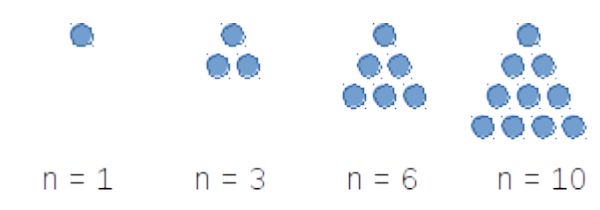
\includegraphics[width=2.7in]{../../resources/images/triangle.png}
\end{center}
Design a circuit that takes four inputs $x_0, x_1, x_2, x_3$ and outputs
True (T or 1) if the integer value 
$(x_3x_2x_1x_0)_{2,4} $ is a triangular number, and False (F or 0) otherwise. You may assume that 0 is
not a triangular number. ({\it Credit: UBC Department of Computer Science})

\ifsolution{
\sol{
Using the definition, we can write a table of values for the circuit we need to build, since the output will be 
one when $(x_3 x_2 x_1 x_0)_{2,4}$ will be one of $1, 3, 6, 10, 15$.
\begin{center}
\begin{tabular}{cccc||c}
$x_3$& $x_2$ & $x_1$ & $x_0$ & Output \\
\hline
$1$ & $1$ & $1$ & $1$ & $1$ \\
$1$ & $1$ & $1$ & $0$ & $0$ \\
$1$ & $1$ & $0$ & $1$ & $0$ \\
$1$ & $1$ & $0$ & $0$ & $0$ \\
$1$ & $0$ & $1$ & $1$ & $0$ \\
$1$ & $0$ & $1$ & $0$ & $1$ \\
$1$ & $0$ & $0$ & $1$ & $0$ \\
$1$ & $0$ & $0$ & $0$ & $0$ \\
$0$ & $1$ & $1$ & $1$ & $0$ \\
$0$ & $1$ & $1$ & $0$ & $1$ \\
$0$ & $1$ & $0$ & $1$ & $0$ \\
$0$ & $1$ & $0$ & $0$ & $0$ \\
$0$ & $0$ & $1$ & $1$ & $1$ \\
$0$ & $0$ & $1$ & $0$ & $0$ \\
$0$ & $0$ & $0$ & $1$ & $1$ \\
$0$ & $0$ & $0$ & $0$ & $0$ \\
\end{tabular}
\end{center}
The output can be described using a compound proposition in DNF with five clauses (because there 
are five rows with output $1$): 
\begin{align*}
&(x_3 \land x_2 \land x_1 \land x_0) \vee (x_3 \land \neg x_2 \land x_1 \land \neg x_0) \vee
(\neg x_3 \land x_2 \land x_1 \land \neg x_0) \\
&\vee (\neg x_3 \land \neg x_2 \land x_1 \land x_0) \vee
(\neg x_3 \land \neg x_2 \land \neg x_1 \land x_0)
\end{align*}
We can use this DNF to draw a circuit that takes the four inputs and whose output is described.

Alternatively, a  logically equivalent compound proposition is
\[
output = \left [ x_1 \wedge ( x_0 \oplus x_2) \oplus x_3 \right] \vee \left [ \neg x_3 \wedge \neg x_2 \wedge \neg x_1 \wedge x_0 \right]
\]

Using this compound proposition, we can draw a circuit with fewer gates than the one described above.

Note: we didn't include picture of circuits in these sample solutions; 
please come to office hours or post to Piazza if you'd like to get feedback 
on a circuit you draw.
}}
\fi


\item[5. Circuits, Compound Propositions, Logical Equivalence] \qquad \\
\begin{enumerate}%[(a)]
\item Draw a logic circuit that uses 
{\bf exactly three} gates and is logically equivalent to
\[
q \leftrightarrow (p \wedge r)
\]
You may (only) use AND, OR, NOT, and XOR gates.

\ifsolution{
\sol{
Since XOR gates are available, we can use a convenient relationship between XOR and $\leftrightarrow$:
\[
q \leftrightarrow (p \wedge r) \equiv \neg ( q \oplus (p \land r) )
\]
Implementing this compound proposition as a circuit, we will use one XOR gate, one AND gate, and
one NOT gate, as required.

Note: we didn't include picture of circuits in these sample solutions; 
please come to office hours or post to Piazza if you'd like to get feedback 
on a circuit you draw.
}}
\fi


\item Write a compound proposition which is logically equivalent to
\[
(p \oplus q) \leftrightarrow r
\] 
You may only use the logical operators negation ($\neg$),
conjunction $(\wedge)$, and disjunction $(\vee)$.

\ifsolution{
\sol{ We apply several logical equivalences in turn: first, we can rewrite $\leftrightarrow$ in terms of 
$\land$ and $\to$:
\[
(p \oplus q) \leftrightarrow r \equiv (~ (p \oplus q) \to r~) \land (~r \to (p \oplus q)~)
\]
Now, we replace $\to$ by its equivalent disjunctive form: $HYP \to CONC \equiv (\neg HYP) \vee CONC$.
Thus, 
\[
(~ (p \oplus q) \to r~) \land (~r \to (p \oplus q)~) \equiv (~ \neg (p \oplus q) \vee r~) \land (~\neg r \vee (p \oplus q)~)
\]
Last, we replace the XOR with equivalent compound propositions in terms of the other connectives:
the XOR is true means one of its inputs is T and the other F; the XOR is false means its inputs are both T or both F.
\begin{align*}
&  (~ \neg (p \oplus q) \vee r~) \land (~\neg r \vee (p \oplus q)~) \equiv \\
&(~ ( (p \land q) \vee (\neg p \land \neg q) ) \vee r~) \land (~\neg r \vee ( ( p \land \neg q) \vee (\neg p \land q)) ~)
\end{align*}
}}
\fi

\item Find a compound proposition that is in DNF (disjunctive normal form) and is logically equivalent
to 
\[
(p \vee q \vee \neg r) \wedge (p \vee \neg q \vee r ) \wedge (\neg p \vee q \vee r)
\]

\ifsolution{
\sol{
The given compound proposition is in CNF and indicates that the rows in the truth table 
with $p=F, q=F, r = T$, $p=F, q= T, r= F$, and $p =T, q=F, r=F$ are set to F.  Thus, the truth table is 

\begin{center}
\begin{tabular}{ccc||c}
$p$ & $q$ & $r$ & Output \\
\hline 
$T$ & $T$ & $T$& $T$ \\
$T$ & $T$ & $F$& $T$ \\
$T$ & $F$ & $T$& $T$ \\
$T$ & $F$ & $F$& $F$ \\
$F$ & $T$ & $T$& $T$ \\
$F$ & $T$ & $F$& $F$ \\
$F$ & $F$ & $T$& $F$ \\
$F$ & $F$ & $F$& $T$ \\
\end{tabular}
\end{center}

To find a logically equivalence compound proposition in DNF, we represent the disjunction
of landing in each of the rows that evaluate to $T$: the rows where
$p =T, q=T, r=T$, or $p=T, q=T, r=F$, or $p=T, q=F, r=T$, or $p=F, q=T, r=T$, or $p=F, q=F, r=F$.
\begin{align*}
(p \land &q \land r)  \vee ( p \land q \land \neg r) \vee (p \land \neg q \land r) \\
&\vee (\neg p \land q \land r) \vee (\neg p \land \neg q \land \neg r)
\end{align*}
}}
\fi

\end{enumerate}

\item[6. Translating Propositional Logic]  \qquad \\

\begin{multicols}{2}
  \begin{itemize}
  \item[] $p$ is ``The display is 13.3-inch"
  \item[] $r$ is ``There is at least 128GB of flash storage"
  \item[] $u$ is ``There is at least 512GB of flash storage"
  \columnbreak
  \item[] $q$ is ``The processor is 2.2 GHz"
  \item[] $s$ is ``There is at least 256GB of flash storage"
  \end{itemize}
\end{multicols}
  
\begin{enumerate}%[(a)]
\item Are the statements 
\[
p \to (r \vee s \vee u) \qquad, \qquad
q \to (s \vee u) \qquad, \qquad
p \leftrightarrow q
\qquad, \qquad \neg u
\]
consistent?  If so, translate to English a possible assignment of truth values to the input propositions
that makes all four statements true simultaneously.

\ifsolution
\sol{
Yes, these statements are consistent.  Consider the assignment of truth values
\[
p = T \qquad q = T \qquad r = T \qquad s = T \qquad u = F
\]
We evaluate the four compound propositions at this assignment to confirm that it makes 
all of them true simulatneously:
\begin{align*}
p \to (r \vee s \vee u) & = T \to (T \vee T \vee F) = T \to T = T \\
q \to (s \vee u) &= T \to (T \vee F) = T \to T = T \\ 
p \leftrightarrow q &= T \leftrightarrow T = T \\
\neg u & = \neg F = T
\end{align*}
Translating to English, we get ``The display is 13.3-inch, the processor is 2.2GHz, 
there is at least 
128GB of flash storage, there is at least 256GB of flash storage, but there is not at 
least 512GB of flash storage."
}
\else{}
\fi

\item Consider this statement in English: 
\begin{quote}
It's not the case that both the display is 13.3-inch and the processor is 2.2 GHz.
\end{quote}
Determine whether each of the compound propositions below is equivalent to the {\bf negation} of that statement, and justify your answers using either truth tables or other equivalences.

Possible compound propositions:
\begin{itemize}
%\begin{inparaenum}[(I)]
\item $\neg p \vee \neg q$ \qquad
\item $\neg (p \to \neg q)$ \qquad
\item $\neg ( p \wedge q)$ \qquad
\item $(\neg p \leftrightarrow \neg q) \wedge p$
%\end{inparaenum}
\end{itemize}
\ifsolution
\sol{
The sentence can be translated to $\neg ( p \wedge q)$.  Its negation is then
\[
\neg \neg (p \wedge q) ~\equiv~  ( p \wedge q) 
~\equiv~ \neg ( p \to \neg q)
\]
because $A \wedge \neg B \equiv \neg (A \to B)$
so $p \wedge q \equiv \neg (A \to \neg B)$.

This is also equivalent to  $(\neg p \leftrightarrow \neg q) \wedge p$, as we can see from
the last two columns of the the truth 
table below

\begin{center}
\begin{tabular}{cc||c|c|c}
$p$ & $q$ & $(\neg p \leftrightarrow \neg q)$ & $(\neg p \leftrightarrow \neg q) \land p$ & $p \land q$ \\
\hline
$T$ & $T$ & $T$ & $T$ & $T$ \\
$T$ & $F$ & $F$ & $F$ & $F$ \\
$F$ & $T$ & $F$ & $F$ & $F$ \\
$F$ & $F$ & $T$ & $F$ & $F$ \\
\end{tabular}
\end{center}
}
\else{}
\fi

\item Consider the compound proposition 
\[
(p \wedge q) \to (r \vee s \vee u)
\]
Express the {\bf contrapositive} of this conditional as a compound proposition.

Then, give an assignment of truth values to each of the input propositional variables
for which the original compound proposition is True but its {\bf converse} is False.

\ifsolution
\sol{
The contrapositive of this conditional 
is 
\[
\neg (r \vee s \vee u) \to \neg (p \land q)
\]
The converse of the original conditional is
\[
(r \vee s \vee u) \to (p \land q)
\]
Consider the assignment of truth values
\[
p = T \qquad q = F \qquad r = T \qquad s = F \qquad u = F
\]
We evaluate the original conditional and its converse with this assignment of truth values:
\begin{align*}
\textrm{Original}: (p \wedge q) \to (r \vee s \vee u) &= (T \wedge F) \to (T \vee F \vee F) = F \to T = T \\
\textrm{Converse}: (r \vee s \vee u) \to (p \wedge q) &= (T \vee F \vee F) \to (T \wedge F) = T \to F = F 
\end{align*}
}
\else{}
\fi
\end{enumerate}


\item[7. Evaluating predicates, Evaluating nested predicates] \qquad \\
\begin{enumerate}%[(a)]
\item Over the domain $\{ 1,2,3,4,5\}$ give an example of predicates $P(x), Q(x)$
which demonstrate that 
\[
(\forall x P(x)) \vee (\forall x Q(x))
\qquad \text{is not logically equivalent to} \qquad 
 \forall x  (~ P(x) \vee Q(x) ~)
\]

\ifsolution
\sol{
We will define  predicates which  make one of  the  statements False and the other  True.
Consider
\begin{center}
\begin{tabular}{c||c||c}
$x$ & $P(x)$  & $Q(x)$ \\
\hline
$1$ & T &  F \\
$2$ & F &  T \\
$3$ & T &  F \\
$4$ & F &  T \\
$5$ & T &  F \\
\end{tabular}
\end{center}
Evaluating the statements: $\forall x (P(x) \vee Q(x))$ is True because each row in the table
has  at  least one  of $P(x)$, $Q(x)$  evaluate  to True.  On the other hand,  neither $\forall x P(x)$
nor $\forall x Q(x)$ is True, because each predicate  at least one  domain element where it evaluates
to  False (for counterexamples: $P(2)$ is  False and $Q(1)$  is False).  Since $F \vee  F = F$, 
$(\forall x P(x)) \vee (\forall x Q(x))$ is False. Since there is  some definition of the predicates $P$ and
$Q$ where the two  statements  
\[
(\forall x P(x)) \vee (\forall x Q(x))~~,~~
 \forall x  (~ P(x) \vee Q(x) ~)
\]
evaluate to different  truth values,  they  are  not logically  equivalent
}
\else{}
\fi


\item Over the domain $\{0,1,2\}$, give an example of predicates $P(x), Q(x)$
for which all of these statements are true:
$$\forall x (P(x) \to Q(x))$$
$$\exists x \, P(x)$$
$$\exists x \, \neg P(x)$$
$$\exists x \, \neg Q(x)$$

\ifsolution
\sol{
We will define  predicates using their  tables  of  values:
\begin{center}
\begin{tabular}{c||c||c}
$x$ & $P(x)$  & $Q(x)$ \\
\hline
$0$ & T &  T \\
$1$ & F &  T \\
$2$ & F &  F \\
\end{tabular}
\end{center}
We  now prove  that each  of the statements is True:
\begin{itemize}
\item To prove  the universal  statement $\forall x (P(x) \to Q(x))$, we  evaluate  the conditional  
at each element in the domain: At  $0$,  $P(0)  \to Q(0) = T \to T = T$;  at $1$,  $P(1) \to Q(1) = F \to T =  T$; 
at $2$,  $P(2) \to Q(2) = F \to F =  T$.   Since the body of the quantification is True at  all element 
in the domain,  $\forall x  (P (x) \to Q(x))$ is True.
\item  To prove the  existential  statement $\exists x P(x)$, we need a witness  in  the  domain where
$P(x)$  evaluates to  True.  The witness is $0$, since the first row in the definition table gives $P(0) = T$.
\item  To prove the  existential  statement $\exists x \neg P(x)$, we need a witness  in  the  domain where
$\neg P(x)$  evaluates to  True.  The witness is $1$, since the second row in the definition table gives $P(1) = F$ so $\neg P(1) = T$.
\item  To prove the  existential  statement $\exists x \neg Q(x)$, we need a witness  in  the  domain where
$\neg Q(x)$  evaluates to  True.  The witness is $2$, since the third row in the definition table gives $Q(2) = F$ so $\neg Q(2) = T$.

\end{itemize}
}
\else{}
\fi

\end{enumerate}

\item[8. Evaluating predicates, Evaluating nested predicates]  Recall that $S$ is defined as the set of all RNA strands, 
where each strand is a nonempty string made of the bases in 
 $B = \{\A,\U,\G,\C\}$. Recall the definition of the following predicates: $F_{\A}$ with domain $S$ is defined recursively by: 
\begin{itemize}
\item[]Basis step: $F_{\A}(\A) = T$, $F_{\A}(\C) = F_{\A}(\G) = F_{\A}(\U) = F$
\item[]Recursive step: If $s \in S$ and $b \in B$, then $F_{\A}(sb) = F_{\A}(s)$
\end{itemize}

$P_{\A\U\C}$ with domain $S$ is defined as the predicate whose truth set
is the collection of RNA strands where the string $\A\U\C$
is a substring (appears inside $s$, in order and consecutively)

$L$ with domain $S \times \mathbb{Z}^+$ is defined by, for $s \in S$ and $n \in \mathbb{Z}^+$,
\[
L( s, n) = \begin{cases}
T &\qquad\text{if $rnalen(s) = n$}\\
F &\qquad\text{otherwise}\\
\end{cases}
\]
\begin{enumerate}%[(a)]
\item Give a witness for $\exists s_1  \, \exists s_2 \,(L(s_1, 4) \land L(s_2,4) \land 
\neg ( s_1 = s_2) )$ where $S$ is
the set of RNA strands, $L(s, n)$ is a predicate with domain $S
\times \mathbb{Z}^+$ that is true when $s$ has length $n$

\ifsolution
\sol{
In English, the statement  can be translated to ``There  are strands $s_1, s_2$ where each has length
$4$ and the strands are not equal."
A witness  is  $s_1 = \C\C\C\C$, $s_2 = \G\G\G\G$.  Since  each of  $s_1, s_2$ is  an element of $S$, 
$s_1$ has  length $4$, $s_2$ has length $4$ and these two strings are not the same.
} 
\else{}
\fi

\item Give a counterexample that disproves  
$\forall i  \,(\neg L(\A\C\U, i)) $ 

\ifsolution
\sol{
In English, the statement  can be translated to ``No positive integer is the length of  the strand \A\C\U."

A counterexample that helps us  disprove this statement is $3$.  This is a positive integer and
is the length of $\A\C\U$ so  $L(\A\C\U, 3)$ is True, hence $\neg L(\A\C\U, 3)$
is False.}
\else{}
\fi

\item Determine which of the following statements is True or False (you do not need to prove your answer).
\begin{enumerate}%[i.]
\item $\exists n \in \mathbb{Z}^+~ \forall s \in S~ ( P_{\A\U\C}(s) \to \lnot L(s,n) )$

\ifsolution{\sol{In English, this statement is saying that there is a positive integer that is not the length of every
RNA strand with $\A\U\C$.  This is {\bf true}, as we can see with the witness $n = 1$.
}}\fi

\item $\exists n \in \mathbb{Z}^+~ \forall s \in S~ ( P_{\A\U\C}(s) \land \lnot L(s,n) )$

\ifsolution{\sol{In English, this statement is saying that there is a positive integer that is not the length of any
RNA strand and that each RNA strand has $\A\U\C$ as a substring.  This is {\bf false}, because
when we consider any positive integer, we'll be able to find a counterexample strand that does not have $\A\U\C$
as a substring and so makes the conjunction false.
}}\fi

\item $\forall s \in S~\exists n \in \mathbb{Z}^+~ ( P_{\A\U\C}(s) \lor \lnot L(s,n) )$

\ifsolution{\sol{In English, this statement is saying that for each RNA strand we can find
some positive integer so that at least one of ``the strand has $\A\U\C$ as a substring" and ``this number
is not the length of this strand" is true. This is {\bf true}, because given any RNA strand, we can pick a witness
positive integer by choosing a number that is not its length.
}}\fi

\item $\forall s \in S~\exists n \in \mathbb{Z}^+~ (L(s,n) \to \lnot P_{\A\U\C}(s))$

\ifsolution{\sol{In English, this statement is saying that for each RNA strand, there is a witness positive integer
which makes the conditional statement ``if the RNA strand has this length then it does not have \A\U\C~as a substring" 
true. This is {\bf true}, because given any RNA strand, we can pick a witness
positive integer by choosing a number that is not its length which will make the hypothesis of the conditional statement
false and therefor the conditional will be true.
}}\fi\end{enumerate}
\end{enumerate}



\end{description}



\newpage%\documentclass{article}


%\usepackage{amsfonts,amssymb,amsmath,amsthm,color,comment,enumerate, graphicx,euscript,hyperref}
%\usepackage[makeroom]{cancel}
%\usepackage{paralist,listings}

%\setlength{\evensidemargin}{0in}
%\setlength{\oddsidemargin}{0in}
%\setlength{\textwidth}{6.6in}
%\setlength{\textheight}{8.8in}
%\setlength{\topmargin}{0in}
%\setlength{\footskip}{0.45in}
\renewcommand{\baselinestretch}{1}
%\newlength{\saveparindent}
%\setlength{\saveparindent}{\parindent}

% % NOTE(joe): This environment is credit @pnpo (https://tex.stackexchange.com/a/218450)
% \lstnewenvironment{algorithm}[1][] %defines the algorithm listing environment
% {   
%     \lstset{ %this is the stype
%         mathescape=true,
%         frame=tB,
%         numbers=left, 
%         numberstyle=\tiny,
%         basicstyle=\rmfamily\scriptsize, 
%         keywordstyle=\color{black}\bfseries,
%         keywords={,procedure, div, mod, for, to, input, output, return, datatype, function, in, if, else, foreach, while, begin, end, } %add the keywords you want, or load a language as Rubens explains in his comment above.
%         numbers=left,
%         xleftmargin=.04\textwidth,
%         #1 % this is to add specific settings to an usage of this environment (for instnce, the caption and referable label)
%     }
% }
% {}

% \newcommand{\A}[0]{\texttt{A}}
% \newcommand{\U}[0]{\texttt{U}}
% \newcommand{\G}[0]{\texttt{G}}
% \newcommand{\C}[0]{\texttt{C}}

\newif \ifsolution
\solutiontrue
\solutionfalse

\newcommand{\soltwo}[1]{\medskip\fbox{\begin{minipage}{6.5in}{#1}\end{minipage}}\medskip}


\begin{center}
{\Large
CSE 20 Spring 2024\\ 
Practice for Test 2 \ifsolution{\qquad Solutions}\fi}
\end{center}

\thispagestyle{empty}

\ifsolution{}
\else{}
Below are the instructions that will be on the first page of the test package:

\begin{center}
  \begin{minipage}[t]{7in}
  \rule{\linewidth}{2pt}
  \textbf{INSTRUCTIONS --- READ THIS NOW}
  \begin{itemize}
  
  \setlength{\itemsep}{0.025in}
  
  \item  Write your name, PID, current seat number, exam time, 
  and the academic integrity pledge in the indicated space above and 
  on the designated  {\bf answer sheet}.
  We will check for {\bf all} of this identifying information before grading.
  Write your answers in the specified areas, or your work will not be graded. 
  
  \item We will not be answering questions about the exam during the exam period. 
  If any bugs are found in the exam after the exam period, the affected question part(s) will be addressed.
  
  \item  You may use one 8.5"x11", doublesided sheet of notes that you create and bring to the exam room, but no other books, notes, or aids.
  
  \item You may not speak to any other student in the exam room while the exam 
  is in progress (including after you hand in your own exam).  You may not share
  {\bf any information} about the exam with anyone who has not taken it.
  
  \item Turn off and put away all cellphones, calculators, and other electronic devices.
  You may not access any electronic device during the exam period. If you need to leave 
  the room during the exam period, you must leave all electronic devices with an exam proctor.
  
  \item  To receive full credit, your answers must
  be written neatly, legibly, and sufficiently darkly to scan well in the indicated answer box. Your solution will be evaluated both for correctness and clarity.
  Read the instructions for each part carefully to determine what is required for full credit.
  This test has $??$ problems worth a total of $??$ points.
  
  \item This exam is {\bf 45 minutes} long. Read all the problems first before you start 
  working on any of them, so you can manage your time wisely.
  
  \item Please stay seated until the end of the exam period.
  We will collect all exams and note sheets at the {\bf end} of the exam period, to minimize disruption 
  for students who wish to use the full time for the exam. Please show your ID to a proctor when 
  asked.
  
  
  \end{itemize}
  \end{minipage} \hfill
  \end{center}
  \newpage
\fi

\begin{description}

  \item[1. Predicates and Quantifiers] 
  Express each of the following statements symbolically using quantifiers, variables, propositional connectives, 
  and predicates (make sure to define the domain and the meaning of any predicates 
  you introduce). Then, express its negation as a logically equivalent compound 
  proposition without a $\neg$ in front.  Decide whether the statement or its negation is true,
  and prove it.
  
  \begin{enumerate}
  \item[(a)] If $m$ is an integer, $m^2 + m +1$ is odd.
  
  \ifsolution
  \soltwo{
  Define the predicate $D(x)$ to mean ``$x$ is odd" with domain $\mathbb{Z}$.
  
  
  The sentence is then $\forall m \in \mathbb{Z} ( D(m^2 + m + 1))$.
  
  Its negation is $\neg \forall m \in \mathbb{Z} ( D(m^2 + m + 1)) \equiv \exists m ( \neg D(m^2 + m + 1))$.
  
  The original statement is true.
  
  {\bf  Proof} Towards universal generalization, let $m$ be an arbitrary integer.  
  By   definition of odd, {\bf to show}: 
  there is an integer $k$ such 
  that $m^2 + m + 1 = 2k + 1$. Factoring the LHS, $m^2 + m + 1 = m(m+1) + 1$.  
  We proceed  in proof by cases, since $m$ is either even or odd.
  \begin{itemize}
  \item Case 1  {\bf to  show}: $(m$ is even $) \to  D(m^2+m+1)$.  In a direct proof of the conditional, 
   assume $m$ is even and choose $c$ be an integer such that $m = 2c$. 
   {\bf To show}: there is an integer such that $m^2+m+1$  is twice  that integer plus $1$.
  To find a witness  for this existential, we substitute  $m=2c$ and calculate, $m(m+1) = 2c(2c+1) = 2( 2c^2 + c) $.
  Since $2c^2 +c \in \mathbb{Z}$ (by properties of integer addition and multiplication), 
  it is the witness we need, because $2(2c^2+c) +1 =  2c(2c+1) +1 = m(m+1)+1 =  m^2+m+1$.
  \item Case 2 {\bf  to  show}: $(m$ is odd $) \to  D(m^2+m+1)$.  In a direct proof of the conditional, 
   assume $m$ is odd and choose $c$ be an integer such that $m = 2c+1$. 
   {\bf To show}: there is an integer such that $m^2+m+1$  is twice  that integer plus $1$.
  To find a witness  for this existential, we substitute  $m=2c+1$ and calculate, $m(m+1) = (2c+1)(2c+2) = 2( 2c+1)(c+1) $.
  Since $(2c+1)(c+1)\in \mathbb{Z}$ (by properties of integer addition and multiplication), 
  it is the witness we need, because $2(2c+1)(c+1)  + 1=  m(m+1) + 1=  m^2+m+1$.
  \end{itemize}
  
  {\it Alternate proof} Let $m$ be an integer.  WTS that $m^2+m+1 \mod 2 = 1$. 
  Case 1: $m \mod 2 = 0$.  Then by modular arithmetic (Corollary 2 on page 242), 
  \begin{align*}
  (m^2 + m + 1) \mod 2 &= \left( (m \mod 2 ) (m \mod 2) + (m \mod 2) + 1 \right) \mod 2 \\
  & = (0 \cdot 0 + 0 +1 ) \mod 2 = 1
  \end{align*}
  as required.  Case 2: $m \mod 2 = 1$.  Then 
  by modular arithmetic (Corollary 2 on page 242), 
  \begin{align*}
  (m^2 + m + 1) \mod 2 &= \left( (m \mod 2 ) (m \mod 2) + (m \mod 2) + 1 \right) \mod 2 \\
  & = (1 \cdot 1 + 1 +1 ) \mod 2 = 3 \mod 2 = 1
  \end{align*}
  as required.
  }
  \else{}
  \fi
  
  \item[(b)] For all integers $n$ greater than $5$, $2^n-1$ is not prime.
  
  \ifsolution
  \soltwo{
  
  Define the predicate: $P(x)$ to mean ``$x$ is prime" with domain: $\mathbb{Z}$. 
  
  The sentence translates to $\forall n ( n > 5 \to \neg P(2^n - 1) )$.
  
  Its negation is 
  $\neg \forall n  \in \mathbb{Z} ( n > 5 \to \neg P(2^n - 1) ) \equiv \exists n \in  \mathbb{Z} (n > 5 \wedge P(2^n -1))$.
  
  The negation is true: to prove it, we need a  witness integer greater than  $5$ where 
  $2^n-1$ is prime.  Consider $n=7$,  an integer so  in the domain.  Calculating, $2^7 -1 =128-1 =127$.   This is a prime
  number because all integers greater than $1$ and less than $\sqrt{127}$  (namely   $2, 3, 4, 5, 6, 7, 8, 9, 10, 11$)
  are not factors of $127$.
  }
  \else{}
  \fi
  
  
  \item[(c)] If $n$ and $m$ are even integers, then $n - m$ is even.
  
  \ifsolution
  \soltwo{
  Define the predicate $E(x)$ to mean 	``$x$ is even" with domain $\mathbb{Z}$.  Note: this 
  predicate could be expressed symbolically as $\exists k \in  \mathbb{Z} (x=2k)$.
  
  The sentence translates to  $\forall x \in \mathbb{Z} ~\forall y \in \mathbb{Z}~( ( E(x) \wedge E(y) ) \to E(x-y) )$.
  
  Its negation is $$\neg \forall x \in \mathbb{Z} ~\forall y \in \mathbb{Z}~( ( E(x) \wedge E(y) ) \to E(x-y) ) 
  \equiv \exists x\in \mathbb{Z} \exists y \in \mathbb{Z} ( E(x) \wedge E(y) \wedge \neg E(x-y))$$
  
  The original statement is true: Towards universal generalization let $x,y$ be arbitrary integers and
  to show is $( E(x) \wedge E(y) ) \to E(x-y)$. Assume, towards
  a direct proof of the conditional that $x$ and $y$ are both even. We WTS that $x-y$ is even.  By definition of even, 
  there are integers $j, h$ such that $x=2j$ and $y=2h$.  Then $x-y = (2j) - (2h) = 2(j-h)$.
  Choosing the  witness $k=j-h$ (an integer), we have proved that $x - y$ is even.
  }
  \else{}
  \fi
  \end{enumerate}
  
  
  \item[2. Proof strategies] Prove each of the following claims.
  Use only basic definitions and general proof strategies in your proofs; 
  do not use any results proved in class / the textbook as lemmas. You may use basic 
  properties of real numbers that we stated (without proof) in class, e.g. that the difference of two
  integers is an integer.
  \begin{enumerate}
  \item[(a)] The difference of any rational number and any irrational number is irrational.
  
  \ifsolution
  \soltwo{
  {\bf Proof}: Symbolically, to show is:
  \[
  \forall x \in \mathbb{R} \forall y \in \mathbb{R}  (  (x \in \mathbb{Q}  \land  y  \notin \mathbb{Q}) \to  (x-y  \notin  \mathbb{Q}))
  \]
  . Towards universal  generalization,  let $x,y$ be arbitrary  real numbers.
  Proceed in a  proof by  contradiction with  
  \[
  p  = (x \in \mathbb{Q}  \land  y  \notin \mathbb{Q}) \to  (x-y  \notin  \mathbb{Q})  \qquad
  r = y  \in  \mathbb{Q}
  \]
  . To show: $\neg p \to (r  \land \neg  r)$.  
  Assume $\neg p$, that is  $x \in \mathbb{Q}  \land  y  \notin \mathbb{Q} \land  x-y  \in  \mathbb{Q}$.  
  To show: $r \land \neg r$. By definition of conjunction,  each conjunct  is  true  and  $y  \notin \mathbb{Q}$  being true means 
  $\neg (y \in  \mathbb{Q}$ is  true.  Thus,  $\neg  r$ is true, and  to  show is:  $r$.
  By definition of $\mathbb{Q}$, there are integers $a,b,p, q$ with $b \neq 0$ and $q \neq 0$ such that $x = \frac{a}{b}, x-y = \frac{p}{q}$.  Then 
  \[
  y = x- (x-y) = \frac{a}{b} - \frac{p}{q} = \frac{aq - bp}{bq}.
  \]
  By  properties of integer multiplication and subtraction, $aq-bp \in \mathbb{Z}$
  and $bq\in \mathbb{Z}$, and since $b,q$ are both nonzero $bq \neq 0$.  Thus, by definition
  of $\mathbb{Q}$, $y \in \mathbb{Q}$, namely,  $r$.
  Thus, we proved $\neg p \to  (r \land  \neg r)$  and so 
  we conclude that $p$ holds.
  
  }
  \else{}
  \fi
  
  \item[(b)] If $a, b, c$ are integers and $a^2 + b^2 = c^2$, then at least one of $a$ and $b$ is even.
  
  \ifsolution
  \soltwo{
  We prove two helper claims (lemmas) before the proof.
  
  {\bf Lemma 1}: For any integer $x$, if $x^2$ is even , then so is $x$.
  
  {\it Proof of Lemma 1}:  Let $x$ be an arbitrary integer and assume (towards proof by contrapositive)
  that $x$ is not even (hence, odd).  WTS that $x^2$ is also not even.
  By assumption, $x = 2k+1$ for some integer $k$.  Squaring: 
  $x^2 = 4k^2+4k+1 = 2(2k^2+2k) + 1$, and by properties of integer addition
  and multiplication $2k^2 + 2k \in \mathbb{Z}$, so $x^2$ is odd, hence not even. \\
  
  
  {\bf Lemma 2}: For any odd integer $x$, $x^2~\text{\bf mod}~4 = 1$.
  
  {\it Proof of Lemma 2}: Let $x$ be an arbitrary odd integer.  By definition, this means there 
  is an integer, call it $k$, such that $x = 2k+1$.  Squaring: $x^2 = 4k^2 + 4k + 1 = 4( k^2 + k) + 1$.
  Since $k^2 + k \in \mathbb{Z}$, $x^2~\text{\bf mod}~4 = 1$.\\
  
  
  {\bf Proof}: Let $a,b,c$ be arbitrary integers.  To show: $a^2 +  b^2 = c^2  \to (E(a) \vee E(b) )$.
  Towards a contradiction, consider
  \[
  p  =   ( a^2 +  b^2 = c^2)  \to (E(a) \vee E(b) ) \qquad  r= (c^2~\text{\bf mod}~4 = 0)
  \]
  To show:  $\neg p \to  (r \land \neg r)$.  Assume $\neg p$, that is 
  $a^2 + b^2 =c^2$ and $a$ and $b$ are both not even.  
  By properties of even/odd, $a$ and $b$ are both odd.  Thus, by Lemma 2,
  $a^2~\text{\bf mod}~4 = b^2 ~\text{\bf mod}~4 = 1$.  By modular arithmetic,
  $c^2 ~\text{\bf mod}~4 = (a^2  + b^2)~\text{\bf mod}~4 = (1 + 1) ~\text{\bf mod}~4 = 2$.
  Since $2 \neq 0$,  this proves $\neg r$.  To show:  $r$.
  Since $c^2~\text{\bf mod}~4 =  2$, there is an integer, call it $q$, such that $c^2 = 4q + 2 = 2(2q+1)$. Thus,
  $c^2$ is even.  Therefore, applying Lemma 1, $c$ is even.
  By definition, this gives an integer $k$ such that $c = 2k$.  Thus, $c^2 = 4k^2 = 4k^2  +0$
  so $c^2~\text{\bf mod}~4 = 0$, namely $r$. Thus, we proved $\neg p \to  (r \land  \neg r)$  and so 
  we conclude that $p$ holds.
  }
  \else{}
  \fi
  
  \item[(c)] For any integer $n$, $n^2 + 5$ is not divisible by $4$.
  
  \ifsolution
  \soltwo{
  Let $n$ be an arbitrary integer.  Towards proof by cases, notice that 
  $(n~\text{\bf mod}~4 = 0) \lor (n~\text{\bf mod}~4 = 1) \lor (n~\text{\bf mod}~4 = 2) \lor (n~\text{\bf mod}~4 = 3)$
  \begin{itemize}
  \item {\bf Case 1 to show}: $(n~\text{\bf mod}~4 = 0) \to (n^2 + 5 \text{ is not divisible by } 4)$.  
  Assume $(n~\text{\bf mod}~4 = 0)$. Then, by modular arithmetic,
  \[
  (n^2 + 5)~\text{\bf mod}~4 = ((n~\text{\bf mod}~4)^2 + 5~\text{\bf mod}~4)~\text{\bf mod}~ 4= ( 0^2 + 1)~\text{\bf mod}~4 = 1~\text{\bf mod}~4.
  \]
  Since $(n^2 +5) ~\text{\bf mod}~4 \neq 0$, $n^2 + 5$ is not divisible by $4$, as required.
  \item {\bf Case 2 to show}: $(n~\text{\bf mod}~4 = 1) \to (n^2 + 5 \text{ is not divisible by } 4)$.  
  Assume $(n~\text{\bf mod}~4 = 1)$. Then, by modular arithmetic,
  \[
  (n^2 + 5)~\text{\bf mod}~4 = ((n~\text{\bf mod}~4)^2 + 5~\text{\bf mod}~4)~\text{\bf mod}~ 4= ( 1^2 + 1)~\text{\bf mod}~4 = 2~\text{\bf mod}~4.
  \]
  Since $(n^2 +5) ~\text{\bf mod}~4 \neq 0$, $n^2 + 5$ is not divisible by $4$, as required.
  \item {\bf Case 3 to show}: $(n~\text{\bf mod}~4 = 2) \to (n^2 + 5 \text{ is not divisible by } 4)$.  
  Assume $(n~\text{\bf mod}~4 = 2)$. Then, by modular arithmetic,
  \[
  (n^2 + 5)~\text{\bf mod}~4 = ((n~\text{\bf mod}~4)^2 + 5~\text{\bf mod}~4)~\text{\bf mod}~ 4= ( 2^2 + 1)~\text{\bf mod}~4 = 5~\text{\bf mod}~4 = 1
  \]
  Since $(n^2 +5) ~\text{\bf mod}~4 \neq 0$, $n^2 + 5$ is not divisible by $4$, as required.
  \item {\bf Case 4 to show}: $(n~\text{\bf mod}~4 = 3) \to (n^2 + 5 \text{ is not divisible by } 4)$.  
  \[
  (n^2 + 5)~\text{\bf mod}~4 = ((n~\text{\bf mod}~4)^2 + 5~\text{\bf mod}~4)~\text{\bf mod}~ 4= ( 3^2 + 1)~\text{\bf mod}~4 = 10~\text{\bf mod}~4 = 2
  \]
  Since $(n^2 +5) ~\text{\bf mod}~4 \neq 0$, $n^2 + 5$ is not divisible by $4$, as required.
  \end{itemize}
  The proof by cases  is now complete for the arbitrary integer $n$.
  }
  \else{}
  \fi
  \item[(d)] For all positive integers $a,b,c$, if $a \not | bc$ then $a \not | b$. {\scriptsize (The notation
  $a \not | b$ means ``a does not divide b'').}
  
  \ifsolution
  \soltwo{
  Let $a,b,c$ be arbitrary  positive integers.  Assume, towards a proof by contrapositive, that 
  $a |b$.  To show: $a | bc$.  By definition of divisibility, there is an integer $k$ such that
  \[
  b = ak.
  \]
  Multiplying both sides by $c$,
  \[
  bc = (ak) c = a (kc).
  \]
  By properties of integer multiplication, $kc \in \mathbb{Z}$ and so it witnesses 
  $a | bc$, as required.
  }
  \else{}
  \fi
  
  \end{enumerate}
  
  {\bf Bonus}: Watch the video \url{https://www.youtube.com/watch?v=MhJN9sByRS0} and write
  down the statement and one or both of the proofs described using the notation, definitions, and 
  proof strategies from CSE 20. 

  \item[3. Sets]  Prove or disprove each of the following statements.
  \begin{enumerate}
  \item[(a)]  For all sets $A$ and $B$, $\mathcal{P}(A) \cup \mathcal{P}(B) = \mathcal{P}(A \cup B)$.
  
  \ifsolution
  \soltwo{
  False.  A counterexample would be $A = \{1\}, B = \{2\}$.  Then 
  \[
  \mathcal{P}(A) \cup \mathcal{P}(B) = \{ \emptyset, \{1\} \} \cup \{ \emptyset , \{2\} \} = 
  \{ \emptyset, \{1\}, \{2\} \}
  \]
  but
  \[
  \mathcal{P}(A \cup B) = \mathcal{P}(\{1,2\}) = \{ \emptyset, \{1\}, \{2\}, \{1,2\} \}.
  \]
  These sets are not equal because they disagree about membership of $\{1,2\}$.
  }
  \else{}
  \fi
  
  \item[(b)] For all sets $A$ and $B$, $\mathcal{P}(A) \cap \mathcal{P}(B) = \mathcal{P}(A \cap B)$.
  
  \ifsolution
  \soltwo{
  True.  Proof: let $A, B$ be arbitrary sets.  We WTS that 
  $\mathcal{P}(A) \cap \mathcal{P}(B) \subseteq \mathcal{P}(A \cap B)$
  and $\mathcal{P}(A \cap B) \subseteq \mathcal{P}(A) \cap \mathcal{P}(B)$.
  \begin{itemize}
  \item[(c)] For the first subset inclusion, consider arbitrary $X \in \mathcal{P}(A) \cap \mathcal{P}(B)$.
  By definition of intersection, $X\in \mathcal{P}(A)$ and $X \in \mathcal{P}(B)$.
  By definition of power set, this means that $X \subseteq A$ and $X \subseteq B$.
  WTS that $X \subseteq A \cap B$: let $x \in X$.  Since $X \subseteq A$, $x \in A$.
  Since $X \subseteq B$, $x \in B$.  Thus, $x \in A$ and $x \in B$ so $x \in A \cap B$.
  Since $x$ was arbitrary, $\forall x ( x \in X \to x \in A \cap B)$ so $X \subseteq A \cap B$.
  Therefore, by definition of power set $X \in \mathcal{P}(A \cap B)$, as required.
  
  \item[(d)] For the second subset inclusion, consider arbitrary $X \in \mathcal{P}(A \cap B)$.  
  By definition of power set, $X \subseteq (A \cap B)$.  WTS that $X \subseteq A$ and 
  $X \subseteq B$.  Let $x \in X$.  Then by definition of subsets, $x \in A \cap B$. 
  By definition of intersection, $x \in A$ and $x \in B$.  Thus $X \subseteq A$ and 
  $X \subseteq B$ and so by definition of power set, $X \in \mathcal{P}(A)$
  and $X \in \mathcal{P}(B)$.  By definition of intersection, $X \in \mathcal{P}(A) \cap 
  \mathcal{P}(B)$, 
  as required.
  \end{itemize}
  }
  \else{}
  \fi
  
  \item[(e)] For any sets $A, B, C, D$,  if the Cartesian products $A\times B$
  and $C \times D$ are disjoint then either $A$ and $C$ are disjoint 
  or $B$ and $D$ are disjoint (or both).
  
  \ifsolution
  \soltwo{
  True.  Proof:  Let $A, B, C, D$ be arbitrary sets.  Towards a proof by contrapositive, 
  we assume that $A \cap C \neq \emptyset$ and $B \cap D \neq \emptyset$ and 
  WTS that $(A \times B) \cap (C \times D) \neq \emptyset$. Since $A \cap C \neq \emptyset$,
  let $x \in A \cap C $.  Since $B \cap D \neq \emptyset$, let $y \in B \cap D$.  
  Let's consider $(x,y)$.  By definition of intersection, since $x \in A \cap  C$
  and $y \in B \cap D$, $x \in A$ and $y \in B$.  Thus, by definition of Cartesian product,
  $(x,y) \in A \times B$.   Similarly, $(x,y) \in C \times D$.  Thus, by definition of intersection, 
  $(x,y) \in (A \times B) \cap (C \times D)$.  In particular, this means that 
  $(A \times B) \cap (C \times D) \neq \emptyset$, as required.
  }
  \else{}
  \fi
  
  \item[(f)] There are sets $A, B$ such that $A \in B$ and $A \subseteq B$.
  
  
  \ifsolution
  \soltwo{
  True.  Proof:  Consider the example $A = \{ 1, 2 \} $ and $B = \{ 1, 2, \{1,2\} \}$. 
  Then $A \in B$ because it ($\{1,2\}$) shows up in the list of elements of $B$.
  Moreover, since each of the elements of $A$ (the numbers $1$ and $2$) are also
  elements of $B$ (they each show up in $B$'s list of elements), $A$ is a subset of $B$.
  }
  \else{}
  \fi
  
  
  \item[(g)] For all sets $A, B, C$: $A \cap B = \emptyset$ and $B \cap C = \emptyset$
  if and only if  $(A \cap B) \cap C = \emptyset$.
  
  \ifsolution
  \soltwo{
  False. Proof:  Consider the counterexample $A = \{ 1, 2 \} $ and $B = \{ 2,3\}$ and
  $C = \{ 3\}$.  Then it is not the case that ``$A \cap B = \emptyset$ and $B \cap C = \emptyset$"
  because $A \cap B = \{ 2\}$.  However, it is the case that $(A \cap B) \cap C = \emptyset$
  because
  \[
  (A \cap B) \cap C = (\{1,2 \} \cap \{ 2,3\} ) \cap \{3\} = \{2\} \cap \{3\} = \emptyset.
  \]
  The biconditional statement is false because one of its arguments is false while the
  other is true.
  }
  \else{}
  \fi
  
  
  \end{enumerate}
  
  
  \item[4. Induction and Recursion] 
  
  Prove the following statements:
  
  \begin{enumerate}
  
  \item[(a)] $\forall s \in S \, (~rnalen(s) = basecount(s,\A) + basecount(s,\C) + basecount(s,\U) + basecount(s,\G)~)$ where $S$ RNA strands and the functions $rnalen$ and $basecount$ are define recursively as: 
  \hspace{-1in}
  \[
  \begin{array}{llll}
  & & \textit{rnalen} : S & \to \mathbb{Z}^+ \\
  \textrm{Basis Step:} & \textrm{If } b \in B\textrm{ then } & \textit{rnalen}(b) & = 1 \\
  \textrm{Recursive Step:} & \textrm{If } s \in S\textrm{ and }b \in B\textrm{, then  } & \textit{rnalen}(sb) & = 1 + \textit{rnalen}(s)
  \end{array}
  \]
  \[
  \begin{array}{llll}
  & & \textit{basecount} : S \times B & \to \mathbb{N} \\
  \textrm{Basis Step:} &  \textrm{If } b_1 \in B, b_2 \in B & \textit{basecount}(b_1, b_2) & =
          \begin{cases}
              1 & \textrm{when } b_1 = b_2 \\
              0 & \textrm{when } b_1 \neq b_2 \\
          \end{cases} \\
  \textrm{Recursive Step:} & \textrm{If } s \in S, b_1 \in B, b_2 \in B &\textit{basecount}(s b_1, b_2) & =
          \begin{cases}
              1 + \textit{basecount}(s, b_2) & \\
              \qquad \textrm{when } b_1 = b_2 &\\
              \textit{basecount}(s, b_2) & \\
              \qquad \textrm{when } b_1 \neq b_2 &\\
          \end{cases}
  \end{array}
  \]
  
  \ifsolution
  \soltwo{
  We proceed by structural induction:
  \begin{itemize}
  \item Basis step: We consider the four cases of $b \in \{ \A, \C, \U, \G \}$, in each to 
  show is that $rnalen(b) = basecount(b,\A) + basecount(b,\C) + basecount(b,\U) + basecount(b,\G)$.
  \[
  rnalen(\A) = 1 \qquad\text{by the basis step in the recursive definition of $rnalen$}
  \]
  \[
  basecount(\A,\A) + basecount(\A,\C) + basecount(\A,\U) + basecount(\A,\G) = 1 + 0 + 0 + 0 = 1
  \]
  by the basis step in the recursive definition of $basecount$, where the first term is the case where 
  $b_1 = b_2 = \A$ and the other three terms are the case where $b_1 \neq b_2$. Thus, 
  $rnalen(\A)  = 1 = basecount(\A,\A) + basecount(\A,\C) + basecount(\A,\U) + basecount(\A,\G)$.
  
  Similarly, 
  \[
  rnalen(\C) = 1 \qquad\text{by the basis step in the recursive definition of $rnalen$}
  \]
  \[
  basecount(\C,\A) + basecount(\C,\C) + basecount(\C,\U) + basecount(\C,\G) = 0 + 1 + 0 + 0 = 1
  \]
  by the basis step in the recursive definition of $basecount$, where the second term is the case where 
  $b_1 = b_2 = \C$ and the other three terms are the case where $b_1 \neq b_2$. Thus, 
  $rnalen(\C)  = 1 = basecount(\C,\A) + basecount(\C,\C) + basecount(\C,\U) + basecount(\C,\G)$; 
  \[
  rnalen(\U) = 1 \qquad\text{by the basis step in the recursive definition of $rnalen$}
  \]
  \[
  basecount(\U,\A) + basecount(\U,\C) + basecount(\U,\U) + basecount(\U,\G) = 0 + 0 + 1+ 0 = 1
  \]
  by the basis step in the recursive definition of $basecount$, where the third term is the case where 
  $b_1 = b_2 = \U$ and the other three terms are the case where $b_1 \neq b_2$. Thus, 
  $rnalen(\U)  = 1 = basecount(\U,\A) + basecount(\U,\C) + basecount(\U,\U) + basecount(\U,\G)$; 
  \[
  rnalen(\G) = 1 \qquad\text{by the basis step in the recursive definition of $rnalen$}
  \]
  \[
  basecount(\G,\A) + basecount(\G,\C) + basecount(\G,\U) + basecount(\G,\G) = 0 + 0 + 0 +1= 1
  \]
  by the basis step in the recursive definition of $basecount$, where the last term is the case where 
  $b_1 = b_2 = \G$ and the other three terms are the case where $b_1 \neq b_2$. Thus, 
  $rnalen(\G)  = 1 = basecount(\G,\A) + basecount(\G,\C) + basecount(\G,\U) + basecount(\G,\G)$.
  The basis step is now complete.
  \item Recursive step: Consider an arbitrary strand $s$ and an arbitrary base $b$.  
  Assume, as the {\bf induction hypothesis} that 
  \[
  rnalen(s) = basecount(s,\A) + basecount(s,\C) + basecount(s,\U) + basecount(s,\G)
  \]
  (continued next page)
  \end{itemize}
  }
  
  \fi
  \ifsolution
  \soltwo{
  
  \begin{itemize}
  \item (Recursive step, continued).  
  We need to show that 
  \[
  rnalen(sb) = basecount(sb,\A) + basecount(sb,\C) + basecount(sb,\U) + basecount(sb,\G)
  \]
  
  We consider the four cases of $b \in \{ \A, \C, \U, \G \}$. In each case, the LHS of the to show is
  \[
  rnalen(sb) = 1 + rnalen(s) \qquad\text{by the recursive step in the  definition of $rnalen$}
  \]
  For the RHS, when $b = \A$:
  \begin{align*}
  RHS = &basecount(s\A,\A) + basecount(s\A,\C) + basecount(s\A,\U) + basecount(s\A,\G) \\
  = &(1 + basecount(s,\A)) + basecount(s,\C) +basecount(s,\U) + basecount(s,\G) \\
  = &1 + ( basecount(s,\A)) + basecount(s,\C) +basecount(s,\U) + basecount(s,\G) ) \\
  = &1 + rnalen(s)  \qquad \text{by the induction hypothesis}
  \end{align*}
  (where the first equation listed is by the recursive step in the definition of basecount, the first term 
  from the case $b_1 = b_2 = \A$  and the rest of the terms from the case $b_1 \neq b_2)$).
  Thus, 
  $LHS = rnalen(s\A)  = 1+ rnalen(s) = RHS$.
  
  Similarly, when $b = \C$:
  \begin{align*}
  RHS = &basecount(s\C,\A) + basecount(s\C,\C) + basecount(s\C,\U) + basecount(s\C,\G) \\
  = &basecount(s,\A) + ( 1+ basecount(s,\C) ) +basecount(s,\U) + basecount(s,\G) \\
  = &1 + rnalen(s)  \qquad \text{by the induction hypothesis}
  \end{align*}
  (where the first equation listed is by the recursive step in the definition of basecount, the second term 
  from the case $b_1 = b_2 = \C$  and the rest of the terms from the case $b_1 \neq b_2)$).
  Thus, 
  $LHS = rnalen(s\C)  = 1+ rnalen(s) = RHS$. When $b = \U$:
  \begin{align*}
  RHS = &basecount(s\U,\A) + basecount(s\U,\C) + basecount(s\U,\U) + basecount(s\U,\G) \\
  = &basecount(s,\A) + basecount(s,\C) + ( 1 + basecount(s,\U)) + basecount(s,\G) \\
  = &1 + rnalen(s)  \qquad \text{by the induction hypothesis}
  \end{align*}
  (where the first equation listed is by the recursive step in the definition of basecount, the third term 
  from the case $b_1 = b_2 = \U$  and the rest of the terms from the case $b_1 \neq b_2)$).
  Thus, 
  $LHS = rnalen(s\U)  = 1+ rnalen(s) = RHS$. Finally, for $b = \G$:
  \begin{align*}
  RHS = &basecount(s\G,\A) + basecount(s\G,\C) + basecount(s\G,\U) + basecount(s\G,\G) \\
  = &basecount(s,\A) + basecount(s,\C)  + basecount(s,\U) + ( 1+ basecount(s,\G) )\\
  = &1 + rnalen(s)  \qquad \text{by the induction hypothesis}
  \end{align*}
  (where the first equation listed is by the recursive step in the definition of basecount, the last term 
  from the case $b_1 = b_2 = \G$  and the rest of the terms from the case $b_1 \neq b_2)$).
  Thus, 
  $LHS = rnalen(s\G)  = 1+ rnalen(s) = RHS$.
  
  \end{itemize}
  
  Since the basis step and recursive steps are complete, we have proved that the equation holds
  for all RNA strands.
  }
\fi

\item[(b)] $\forall l_1 \in L \, \forall l_2 \in L \, (\textit{sum}(\textit{concat}(l_1, l_2)) = \textit{sum}(l_1) + \textit{sum}(l_2))$, where the function $\textit{concat}$ is defined as:
\[
\begin{array}{llll}
& & \textit{concat} : L \times L & \to L \\
\textrm{Basis Step:} & \textrm{If } l \in L & \textit{concat}([], l) & = l \\
\textrm{Recursive Step:} & \textrm{If } l, l' \in L\textrm{ and }n \in \mathbb{N}\textrm{, then  } & \textit{concat}((n, l), l') & = (n, \textit{concat}(l, l'))
\end{array}
\]
and the function $\textit{sum} : L \to \mathbb{N}$ that sums all the elements of a list and is defined by:
\[
\begin{array}{llll}
& & \textit{sum} : L & \to \mathbb{N} \\
\textrm{Basis Step:} & & \textit{sum}([]) & = 0 \\
\textrm{Recursive Step:} & \textrm{If } l \in L, n \in \mathbb{N} & \textit{sum}((n, l)) & = n + \textit{sum}(l)
\end{array}
\]

\ifsolution
\soltwo{
We proceed by structural induction on $l_1$ by definition of $L$.
\begin{itemize}
\item Basis step: To show is that $\forall l_2 \in L \, (\textit{sum}(\textit{concat}([], l_2)) = \textit{sum}([]) + \textit{sum}(l_2))$. We proceed by universal generalization and let $l_2$ be an arbitrary element of $L$. By definition of \textit{concat}, we can rewrite the To Show as $\textit{sum}(l_2) = \textit{sum}([]) + \textit{sum}(l_2)$. By definition of \textit{sum}, we can rewrite the right-hand side as $0 + \textit{sum}(l_2)$. This shows that our goal can be rewritten to $\textit{sum}(l_2) = \textit{sum}(l_2)$, which is true.
\item Recursive step: To show is that $\forall l_2 \in L \, (\textit{sum}(\textit{concat}((n, l_1'), l_2)) = \textit{sum}((n, l_1')) + \textit{sum}(l_2))$, where $n \in \mathbb{N}$ and $l_1' \in L$. We assume as the inductive hypothesis that $\forall l_2 \in L \, (\textit{sum}(\textit{concat}(l_1', l_2)) = \textit{sum}(l_1') + \textit{sum}(l_2))$.

We proceed by universal generalization and assume that $l_2$ is an arbitrary element of $L$. Applying the definition of \textit{concat}, we can rewrite To Show as $$\textit{sum}((n, \textit{concat}(l_1', l_2))) = \textit{sum}((n, l_1')) + \textit{sum}(l_2)$$. We can further apply the definition of \textit{sum} on both sides to rewrite To Show as: $$n + \textit{sum}(\textit{concat}(l_1', l_2))) = n + \textit{sum}(l_1') + \textit{sum}(l_2)$$. By the rules of arithmetic on $+$, this is true when $$\textit{sum}(\textit{concat}(l_1', l_2))) = \textit{sum}(l_1') + \textit{sum}(l_2)$$. Since $l_2 \in L$, we can apply the inductive hypothesis, whose body exactly matches this goal.

\end{itemize}
}
\fi

\end{enumerate}


\item[5. Induction and Recursion] 
At time 0, a particle resides at the point 0 on the real line.  
Within 1 second, it divides into 2 particles that fly in opposite directions and 
stop at distance 1 from the original particle. Within the next second, 
each of these particles again divides into 2 particles flying in opposite directions 
and stopping at distance 1 from the point of division, and so on. 
Whenever particles meet they annihilate (leaving nothing behind). 
How many particles will there be at time $2^{11} -1$? 
You do not need to justify your answer. 
Hint: Derive a formula for the number/ locations of particles at time $2^n-1$ for arbitrary 
positive integer n, prove the formula using induction, and apply it when $n=11$.

\ifsolution
\soltwo{\qquad  {\bf $2^{11}$ particles}  \qquad

  Proof: We will prove by mathematical induction that, 

  \begin{quote}
    For each positive integer $n$, a particle that 
    started at time $0$ in position $0$ has the 
    property that between time $0$ and time $2^n-1$, 
    it and all of its descendants have stayed in the 
    interval $[-2^n+1, 2^n-1]$ and at time $2^n-1$, its descendants are located exactly
    on each odd location in $[-2^{n}+1,2^n-1]$ (inclusive).
  \end{quote}
  
  {\it How to use this lemma?} 
  Substituting $n = 11$, this lemma says that at time $2^{11}-1$, the
  descendants of the original particle are located at odd each location in 
  the interval $[-2^{11}+1, 2^{11}-1]$ (inclusive).  Therefore, the number of 
  particles at this time is the number of odd integers in the interval.
  There are $\lceil \frac{2^{11}-1}{2} \rceil = \frac{2^{11}}{2} = 2^{10}$ many 
  such negative odd integers, 
  and $\lceil \frac{2^{11}-1}{2} \rceil =\frac{2^{11}}{2} = 2^{10}$   
  many such positive odd integers, so a total 
  of $2^{10}+2^{10} = 2^{11}$ particles.\\
  
  To prove the lemma, we proceed by mathematical induction.

  \begin{itemize}
    \item {\bf Basis step} For $n=1$, we WTS that between time $0$ and
      time $2^1-1$, the particle and all its descendants have stayed in the interval
      $[-2^1+1, 2^1-1]$, and at time $2^1-1$, there are particles at each odd location
      this interval.  Plugging in $n=1$, we see that the interval is $[-1,1]$ and we WTS that 
      at time $1$ there are particles exactly at the endpoints of this interval (these are 
      the odd locations).  Applying the definition of the process, at time $1$, the original 
      particle divides into two and the two new particles reach distance $1$ from the original.
      This means that the only locations at which particles resided in this interval are
      $0,-1,1$ (all within the required interval) and that at time $1$, the particles
      are at $-1$ and $1$, as required.
  \end{itemize}  
  (continued next page)
  }
\fi
\ifsolution {
\newpage
\soltwo{
  \begin{itemize}
  \item {\bf Induction step} Let $k$ be an arbitrary positive integer.  Assume,
    as the {\bf Induction Hypothesis (IH)}, that
    \begin{quote}
      between time $0$ and time $2^k-1$, 
      the particle and all of its descendants have stayed in the region on the number 
      line $[-2^k+1, 2^k-1]$ and at time $2^k-1$, its descendants are located exactly
      on each odd location in $[-2^{k}+1,2^k-1]$ (inclusive).
    \end{quote}
  
    We WTS that
    \begin{quote}
      between time $0$ and time $2^{k+1}-1$, 
      the particle and all of its descendants have stayed in the region on the number 
      line $[-2^{k+1}+1, 2^{k+1}-1]$ and at time $2^{k+1}-1$, 
      its descendants are located exactly
      on each odd location in $[-2^{k+1}+1,2^{k+1}-1]$ (inclusive).
    \end{quote}
    We'll consider the progress of the experiment through time.  At time step
    $2^k$, one unit of time has elapsed since the situation described in the IH.
    By the setup of the experiment, during this unit of time, each particle splits into
    two and these travel one unit in each axis direction.  Since (by the IH) 
    at time $2^k-1$, there are particles
    at each odd location in the interval $[-2^{k}+1,2^k-1]$, each of these particles
    are two units apart.  Thus, the particles originating from successive
    odd locations in time $2^{k}-1$ will meet and annihilate at time $2^k$. 
    The only particles that will remain at time $2^k$ are (1) the particle that originates
    at time $2^k-1$ from location $-2^k +1$ and goes left and (2) the particle that 
    originates at time $2^k-1$ from location $2^k-1$ and goes right.  Thus, 
    at $2^k$ there are two particles, one at $-2^k$ and the other at $2^k$.
    For definiteness, let's call the particle at position $-2^k$, $p_L$, and the one
    at position $2^k$, $p_R$.    Recalibrating the experiment with position $2^k$ as
    the new ``origin" and particle $p_R$ as our original particle, the IH guarantees that 
    between the current time ($2^k$) and $2^k-1$ steps in the future, $p_R$ will
    divide into particles such that all of its descendants 
    will stay in the interval $[\text{``origin"}-2^{k}+1, \text{``origin"}+2^{k}-1]$ 
    and  its descendants will end up exactly
    on each odd location in $[\text{``origin"}-2^{k}+1, \text{``origin"}+2^{k}-1]$
    (inclusive).  That is, at time $2^k+2^k-1 = 2^{k+1}-1$, the process 
    starting $p_R$ will have generated particles at all odd locations
    in $[0, 2^{k+1}-1]$.  Symmetrically, the IH guarantees that at time $2^{k+1}-1$,
    all descendants of the particle $p_L$  will be at the odd locations in
    $[-2^{k+1}+1, 0]$, and will never have gone beyond that interval at any time 
    since 
    time $2^{k}-1$.  Since the intervals in which the descendants of $p_L$ and 
    $p_R$ land between these timestamps only overlap at $0$, the particles
    generated by these two experiments never collide and so the two 
    experiments run independently.  Thus, at time $2^{k+1}-1$, there
    are $2^k + 2^k = 2^{k+1}$ many particles, occupying each odd location in the interval
    $[-2^{k+1}+1, 0] \cup [0, 2^{k+1}-1] = [-2^{k+1}+1, 2^{k+1}-1]$, and 
    these particles (and their predecessors) have not left this interval at any point 
    up to this time step.  In particular, this means that the lemma is proved.
  \end{itemize} }}
\else{}
\fi

\item[6. Induction and Recursion] 
Prove that every positive integer has a base $3$ expansion. {\it Hint: use strong induction.}

\ifsolution
\soltwo{
By definition of base expansion, we need to prove that for every positive integer $n$, 
there is a positive integer $k$ and nonnegative integers $a_0, a_1, \ldots, a_{k-1}$ 
such that each $a_i \in \{0,1,2\}$, $a_{k-1} \neq  0$, and
\[
n = \sum_{i=0}^{k-1} a_i 3^i
\]
We proceed by strong induction on $n \geq 0$.
\begin{itemize}
\item Basis steps (using the terminology for strong induction: we choose $b=1, j=1$): For the positive integer $1$, we have witnesses
$k=1, a_0 = 1$ and since $1 \in \{0,1,2\}$, $1 \neq 0$, and $1 = \sum_{i=0}^0 a_i 3^i$, the claim
is proved. For the positive integer $2$, we have witnesses
$k=1, a_0 = 2$ and since $2 \in \{0,1,2\}$, $2 \neq 0$, and $2 = \sum_{i=0}^0 a_i 3^i$, the claim
is proved.
\item Recursive step: Consider an arbitrary positive integer $n$ greater than or equal to $2$. 
Assume, as the strong induction induction hypothesis that each positive number less than or equal to $n$ 
has a base $3$ expansion. We need to show that $n+1$ has a base $3$ expansion. To build the required
witnesses, consider the integer $c = (n+1) \textbf{ div } 3$. By properties of integers, since $n+1 \geq 3$
(because $n \geq 2$), $1 \leq c \leq n$.  Thus, the strong induction hypothesis applies to $c$ and there
is a positive integer $k_c$ and nonnegative integers $x_0, x_1, \ldots, x_{k_c-1}$ 
such that each $x_i \in \{0,1,2\}$, $x_{k_c-1} \neq  0$, and
\[
c = \sum_{i=0}^{k_c-1} x_i 3^i
\]
Define $k = k_c + 1$, $a_i = x_{i-1}$ for each $i$ from $1$ to $k$, and $a_0 = (n+1) \textbf{ mod } 3$.
Then $k$ is positive (because $k_c$ is), each $a_i \in \{0,1,2\}$ (because all the $x_i$ are in this
set, and the remainder upon division by $3$ of any positive integer is also in this set), $a_{k-1} =
a_{k_c+1 - 1} = x_{k_c-1} \neq 0$ (by choice of $k$ and definition of $x_i$s). It remains to prove that the 
sum gives the right value: 
\begin{align*}
\sum_{i=0}^{k-1} a_i 3^i &= \left( \sum_{i=1}^{k-1} a_i 3^i \right) + a_0 3^0
=  3 \left( \sum_{i=1}^{(k_c+1)-1} x_{i-1} 3^{i-1} \right) + a_0 3^0
= 3 \left( \sum_{j=0}^{k_c - 1} x_j 3^j \right) + a_0\\
&= 3 c + a_0 = 3 ( (n+1) \textbf{ div } 3) + ( (n+1) \textbf{ mod } 3 ) = n+1
\end{align*}
as required.
\end{itemize}
Since the existence of base $3$ expansions was proved for all positive integers (for $1, 2$ in
the basis cases, and all integers greater than or equal to $3$ in the recursive step), the proof
by strong induction 
is complete.
}
\else{}
\fi



\item[7. Functions \& Cardinalities of sets] Prove each of the following claims.
\begin{enumerate}

\item[(a)] For the ``function" $f: \mathbb{Z} \to \{0, 1, 2, 3 \}$ given by $f(x) = x~\text{\bf mod}~5$, it is not the case that every element of the domain maps to exactly one element of the codomain (that is, it is not a well-defined function).


\ifsolution
\soltwo{
This function is not well defined because $f(4)$ is not in the codomain
even though $4$ is in the domain: 
$f(4) =4~\text{\bf mod}~5 = 4 \notin \{0,1,2,3\}$.
}
\else{}
\fi

\item[(b)] The ``function" $f: \mathcal{P}( \mathbb{Z}^+) \to \mathbb{Z}$ given by 
\[
f(A) = \text{the maximum element in 
A}
\] is not well-defined.

\ifsolution
\soltwo{
This function is not well defined because $f(\mathbb{Z}^+)$ is not well-defined
even though $\mathbb{Z}^+$ is in the domain: 
the set $\mathbb{Z}^+$ doesn't have a maximum element.
}
\else{}
\fi

\item[(c)] There is a one-to-one function with domain $\{a,b,c\}$ and codomain $\mathbb{R}$.

\ifsolution
\soltwo{
Define the function $f:\{a,b,c\} \to  \mathbb{R}$ 
by the piecewise definition
\begin{align*}
f(a) &= 1, f(b) = 2, f(c) = 3
\end{align*}
This function is well-defined because it maps every domain element to a unique output, and
all outputs are in the specified codomain.  Moreover, it is one-to-one: each of the three
distinct domain elements have different images from one another.
}
\else{}
\fi

\item[(d)] There is an onto function with domain $R$ and codomain $\{ \pi, \frac{1}{17} \}$, where $R$ is the set of 
user ratings in a database with 5 movies.

\ifsolution
\soltwo{
Define the function $f: R \to \{\pi, \frac{1}{17} \}$ 
by the piecewise definition
\begin{align*}
f(w) &=  \begin{cases}
\pi \qquad \text{if $w = (0,0,0,0,0)$} \\
\frac{1}{17} \qquad \text{otherwise}
\end{cases}
\end{align*}
This function is well-defined because it maps every ratings $5$-tuple to a unique output, and
all outputs are in the specified codomain.  Moreover, it is onto: we need to confirm
that each element in the codomain has a preimage. Consider, for example
\[
f( (0,0,0,0,0) ) = \pi \qquad f( (1,1,1,1,1) ) = \frac{1}{17}.
\]
}
\else{}
\fi



\item[(e)] The Cartesian product $\mathbb{Z}^+ \times \{ a,b,c \}$ is countable.

\ifsolution
\soltwo{
We rewrite
\[
\mathbb{Z}^+ \times \{ a,b,c \} = \left( \mathbb{Z}^+ \times\{a\} \right) \cup \left( \mathbb{Z}^+ \times\{b\} \right)
\cup \left( \mathbb{Z}^+ \times \{c\} \right) 
\]
Using the function $f: \mathbb{Z}^+ \to \mathbb{Z}^+ \times\{a\}$ given by $f(n) = (n,a)$, 
we can prove that $\mathbb{Z}^+ \times\{a\}$ is countably infinite.  Similarly, 
$\mathbb{Z}^+ \times\{b\}$  and $\mathbb{Z}^+ \times\{c\}$ are countably infinite.
By Theorem 1 on page 174 in the book, $ \left( \mathbb{Z}^+ \times\{a\} \right) \cup \left( \mathbb{Z}^+ \times\{b\} 
\right)$ is countable because it is the union of
two countably infinite (hence countable) sets.  
Applying this theorem again when taking the union of this resulting set
with the set $\left( \mathbb{Z}^+ \times\{c\} \right)$, we see that the set is countable.
}
\else{}
\fi

\item[(f)] The interval of real numbers $\{x \in \mathbb{R}  ~\mid~ 5  \leq x \leq 8\}$ is uncountable.  {\it Hint: you may use
the fact that the unit interval $\{  x \in \mathbb{R} ~\mid~ 0  \leq x \leq  1\}$ is uncountable.}

\ifsolution
{\soltwo{
For brevity, we use the interval notation  $[5,8] = \{x \in \mathbb{R}  ~\mid~ 5  \leq x \leq 8\}$
and  $[0,1] = \{  x \in \mathbb{R} ~\mid~ 0  \leq x \leq  1\}$.
Define the function $f: [0,1] \to [5,8]$ by $f(x) = 5 + 3x$.  Then $f$ is a bijection: 
\begin{itemize}
\item Well-defined? for each $x$ in $[0,1]$, $0 \leq x \leq 1$ so $0 \leq 3x \leq 3$
and $5 \leq 5 + 3x \leq 8$.  Thus, $f(x) \in [5,8]$, as required.
\item Invertible? Consider the function $g:[5,8] \to[0,1]$ defined by $g(x) = \frac{x-5}{3}$.
WTS that for each $x \in [0,1]$, $g(f(x)) = x$ and for each $x \in [5,8]$, $f(g(x)) = x$.
Let $x \in [0,1]$.  Then 
\[
g(f(x)) = g( 5+3x) = \frac{(5+3x) - 5}{3} = \frac{3x}{3} = x,
\]
as required.  Similarly, let $x \in[5,8]$.  Then
\[
f(g(x)) = f ( \frac{x-5}{3}) = 5 + 3 \cdot \frac{x-5}{3} = 5 + (x-5) = x,
\]
as required.  Thus, $f$ is invertible (with inverse $g$) and so is a bijection.
\end{itemize}
}
}
\else{}
\fi

\end{enumerate}

\end{description}



\newpage

\end{document}